\documentclass[12pt,a4paper,twoside,fleqn]{article}
\usepackage[inner=29mm,outer=26mm,top=28mm,bottom=29mm,headheight=16pt]{geometry}
\usepackage[T1]{fontenc}
\usepackage{newtxtext}
\usepackage{amsmath,amsthm,mathtools,newtxmath,microtype}
\usepackage{booktabs,tabularx,array,graphicx,float,enumitem,titlesec,fancyhdr}
\usepackage[round,authoryear]{natbib}
\renewcommand{\bibfont}{\small\raggedright}
\usepackage[hidelinks]{hyperref}
\hypersetup{bookmarksdepth=2}
\urlstyle{same}
\newcommand{\doi}[1]{\href{https://doi.org/#1}{\textnormal{#1}}}
\newcommand{\DOIprefix}{doi:\,}
\pagestyle{fancy}\fancyhf{}
\fancyhead[LE,RO]{\small\thepage}
\fancyhead[LO]{\small Weak-Allee growth and a foraging-arena response}
\fancyhead[RE]{\small Coexistence, stability and bifurcation}
\fancypagestyle{plain}{\fancyhf{}\fancyfoot[C]{\thepage}\renewcommand{\headrulewidth}{0pt}}
\titleformat{\section}{\large\bfseries}{\thesection.}{.65em}{}
\titleformat{\subsection}{\normalsize\itshape}{\thesubsection.}{.65em}{}
\setlength{\mathindent}{1.7em}
\setlength{\emergencystretch}{1.5em}
\setlength{\intextsep}{12pt}
\setlist[enumerate,1]{label=\textup{(\roman*)},leftmargin=2.2em,topsep=4pt,itemsep=3pt}
\setcounter{tocdepth}{1}
\newcolumntype{Y}{>{\raggedright\arraybackslash}X}
\newtheoremstyle{journal}{9pt}{7pt}{\itshape}{}{\bfseries}{.}{.45em}{\thmname{#1}\thmnumber{ #2}\thmnote{ \textup{(#3)}}}
\theoremstyle{journal}
\newtheorem{theorem}{Theorem}
\newtheorem{lemma}{Lemma}
\newtheorem{proposition}{Proposition}
\newtheorem{corollary}{Corollary}
\newcommand{\claim}[1]{{\normalfont\bfseries\boldmath #1}}
\renewcommand{\proofname}{\normalfont\bfseries Proof}
\newcommand{\dd}{\mathrm{d}}
\newcommand{\tr}{\operatorname{tr}}
\newcommand{\Real}{\operatorname{Re}}
\newcommand{\Q}{\mathcal Q}
\newcommand{\Det}{\mathcal D}
\newcommand{\pos}{\mathbb R_{>0}^{\,2}}
\raggedbottom
\begin{document}
\thispagestyle{plain}
{\raggedright\noindent\LARGE\bfseries Proof supplement\par}
\vspace{.5em}
{\raggedright\noindent\large Coexistence, stability, and bifurcation in a predator--prey model with weak Allee growth and a foraging-arena response\par}
\vspace{1em}{\noindent Project 3H (Version B) \textbar\ Companion to the revised report\par}\vspace{1.1em}

This document gives the full mathematical derivations behind the deterministic model in the revised report. Sections~2--7 cover positivity and persistence, equilibria, local and global stability, bifurcations, and enrichment. Section~8 gives analytical diagrams in cubic and normal-form coordinates. The numerical phase portraits and simulation protocols appear in the main report.

The system here is the displayed equation (1.1) of the supplied Version B brief, with the coefficient of the separate predator self-competition term set to zero. In this supplement the Hopf and Bautin parameter \(h\) is the scaled predator equilibrium density \(Y^*\), written \(h_*\) in the revised report. The symbol \(t\) in the focal-coefficient calculation is a dimensionless prey-growth slope, written \(\theta\) in the main report. Physical time elsewhere is \(t\), with \(\tau=rt\).

The group's available Phase~8 record is \texttt{worked report/Research\_Report.pdf} in the supplied project archive. The original derivation also credits a separate internal Task~4 note, which was unavailable in that archive. The prey-floor/entropy argument it motivated is presented directly in Section~\ref{sec:global}. Numbering within this supplement follows the longer derivation.

\tableofcontents
\clearpage
\section{Introduction}
Lotka--Volterra interactions couple predator increase and prey loss through the same encounter term. Logistic prey growth adds density regulation, giving the prey a finite carrying capacity in the absence of predators. We retain that carrying capacity and allow prey per-capita growth to rise initially with density. This is a weak Allee effect because low-density growth remains positive. Predator interference enters through a foraging-arena response whose per-predator intake is linear in prey density and decreases with predator density. The combination raises a question about coexistence that the invasion test alone cannot settle. Once the predator invades, the prey nullcline can support several equilibria and qualitatively different attractors.

\citet{haque09} studied a ratio-dependent predator--prey system, including its boundary dynamics and conditional enrichment effects. The response denominator there mixes prey and predator densities. \citet{haque11} used the Beddington--DeAngelis response with logistic prey growth, studying permanence, global attraction and local bifurcations. Its terms involving prey in the response denominator and additional predator mortality change the Jacobian and the equilibrium equation. The present denominator is positive at the origin, and the prey growth can turn before carrying capacity. The analyses of \citet{hsu01} for a ratio-dependent system and \citet{wang11} for strong Allee growth give methods for limit-set and cycle arguments whose hypotheses must be checked again here. The formulation follows the Version B project brief \citep{brief}.

The questions addressed here are whether invasion ensures persistence, how many coexistence states are feasible, and which branches lead to convergence or oscillation. Section~\ref{sec:local} follows each equilibrium from the two axes to the three coexistence branches. Table~\ref{tab:global} and Section~\ref{sec:globalmap} give the parameter regions with proved long-term outcomes and identify the remaining cycle and basin questions. The bifurcation constructions distinguish the choice of a critical family from the subsequent variation of a single physical parameter.

\section{Model formulation and fundamental properties}\label{sec:model}
Let \(x(t)\) and \(y(t)\) be prey and predator densities, respectively. With strictly positive initial populations the model is
\begin{equation}\label{eq:ode}
 \begin{aligned}
 \frac{\dd x}{\dd t}&=xF(x)-\frac{mxy}{\beta+y}=f(x,y),\\
 \frac{\dd y}{\dd t}&=\frac{emxy}{\beta+y}-dy=g(x,y),\\
 x(0)&=x_0>0,\qquad y(0)=y_0>0,
 \end{aligned}
\end{equation}
Here \(F(x)=r(1-x/k)(1+\alpha x)\), so \(F(0)=r>0\). The condition \(F'(0)>0\) is exactly \(A=\alpha k>1\). If \(A\le1\), \(F\) decreases for positive \(x\), including \(A=1\) when \(F'(0)=0\).

\begin{table}[H]\centering
\caption{Dimensional and dimensionless parameters. All model parameters are positive.}
\label{tab:param}
\begin{tabularx}{\linewidth}{@{}lYl@{}}\toprule
Input & Meaning & Scaled quantity \\ \midrule
\(r\) & Intrinsic prey growth rate & \(\tau=rt\) \\
\(k\) & Prey carrying capacity & \(X=x/k\) \\
\(\alpha\) & Coefficient of density facilitation in prey growth & \(A=\alpha k\) \\
\(m\) & Predation coefficient in the prey per-capita loss & \(M=m/r\) \\
\(\beta\) & Predator density at half-saturation of total intake per prey & \(Y=y/\beta\) \\
\(e\) & Conversion efficiency for prey consumed & \(R=emk/(d\beta)\) \\
\(d\) & Predator mortality rate & \(D=d/r\) \\
\bottomrule
\end{tabularx}
\end{table}

The reversible state and time scaling in Table~\ref{tab:param} gives
\begin{equation}\label{eq:scaled}
 \begin{aligned}
 X'&=X\left[p(X)-\frac{MY}{1+Y}\right],\\
 Y'&=DY\left[\frac{RX}{1+Y}-1\right],\\
 p(X)&=(1-X)(1+AX),
 \end{aligned}
\end{equation}
where prime on state variables denotes \(\dd/\dd\tau\). Given \(r,k,\beta\) and the four scaled parameters, the inverse is \(\alpha=A/k,\ m=rM,\ d=rD,\ e=DR\beta/(Mk)\), with \(x=kX,\ y=\beta Y,\ t=\tau/r\). In particular \(R\) is the predator's per-capita birth-to-death ratio at \((k,0)\).

\begin{theorem}[Positivity, continuation and bounds]\label{thm:bounds}
\claim{The nonnegative quadrant is invariant and the flow is forward complete.} Every nonnegative trajectory exists for all \(t\ge0\), and positive initial data give positive coordinates. With
\[
 W=ex+y,\qquad B_0=\max_{x\ge0} ex[F(x)+d],
\]
one has \(W(t)\le W(0)e^{-dt}+(B_0/d)(1-e^{-dt})\). Also
\[
 x(t)\le\max(x(0),k),\quad \limsup_{t\to\infty}x(t)\le k,\quad
 \limsup_{t\to\infty}y(t)\le\beta\max(0,R-1).
\]
\end{theorem}
\begin{proof}
The vector field is smooth on \(y>-\beta\). Local uniqueness, together with the factors \(x\) and \(y\), makes each axis invariant and forbids finite-time contact from the open quadrant. Equivalently, each population equals its initial value times the exponential of the integral of its continuous per-capita rate. Cancellation gives \(\dot W=-dW+ex[F(x)+d]\). The maximum is finite because the leading cubic coefficient is negative. Integrating the inequality bounds both coordinates and keeps the orbit in a compact subset of the smooth domain on every bounded time interval, giving continuation. The set \(W\le B_0/d+1\) in the quadrant is positively invariant and absorbing. Scalar comparison with \(\dot x=xF(x)\) gives the prey bounds. Eventually \(x\le k+\varepsilon\). Compare the predator to the scalar equation \(\dot z=z[em(k+\varepsilon)/(\beta+z)-d]\), whose nonnegative long-term bound is \(\max(0,em(k+\varepsilon)/d-\beta)\). Let \(\varepsilon\downarrow0\).
\end{proof}

\begin{theorem}[Exact persistence threshold]\label{thm:per}
\claim{Both species are uniformly persistent exactly when \(R>1\).} For positive data and \(R\le1\), \((x(t),y(t))\to(k,0)\). For \(R>1\) there is a parameter-dependent \(\delta_*>0\) such that \(\liminf x,\liminf y\ge\delta_*\) for every positive trajectory.
\end{theorem}
\begin{proof}
Write \(\xi=d\beta/(em)=k/R\). For \(R\le1\), Theorem~\ref{thm:bounds} gives \(y\to0\). For each \(b<k\) with \(b>0\), put \(F_b=\min_{[0,b]}F>0\). Eventually \(\dot x/x\ge F_b/2\) whenever \(x\le b\). Thus \(x\) reaches \(b\) if below and cannot return below it. Let \(b\uparrow k\).

For \(R>1\), fix \(b_0=\xi/2\), \(\gamma=d/2\) and \(\overline y=\beta(2R-1)\). Eventually \(y\le\overline y\). On an excursion below \(b_0\) starting at time \(s\) with \(x(s)=b_0\), \(F(x)>0\) and \(\dot y/y\le-\gamma\). Hence
\[
 \log(x(t)/b_0)\ge-\int_0^\infty
 \frac{m\overline y e^{-\gamma v}}{\beta+\overline y e^{-\gamma v}}\,\dd v
 =-\frac{m}{\gamma}\log(1+\overline y/\beta).
\]
If \(x<b_0\) when the eventual bound first applies, it reaches \(b_0\) in finite time. Otherwise \(y\to0\) there, forcing eventual positive prey growth at rate at least \(F_{b_0}/2\). Thus eventually \(x\ge\delta=b_0(1+\overline y/\beta)^{-m/\gamma}\).

Choose \(b\in(\xi,k)\) and \(\eta>0\) small enough that \(m\eta/(\beta+\eta)<F_b/2\) and \(emb/(\beta+\eta)>d\). Whenever \(y\le\eta\), prey reaches \(b\) within \(L=2\log(b/\delta)/F_b\) if needed and stays above \(b\) while \(y\le\eta\). Thereafter \(y\) grows exponentially until reaching \(\eta\). A first excursion beginning below \(\eta\) therefore ends in finite time. Every later excursion starting at \(\eta\) has \(y\ge\eta e^{-dL}\), by \(\dot y/y\ge-d\) before prey recovery and positive predator growth afterwards. Take \(\delta_*=\min(\delta,\eta e^{-dL})\).
\end{proof}

\section{Equilibria and their complete classification}\label{sec:eq}
\subsection{Boundary equilibria and feasibility}
\begin{lemma}[Feasibility]\label{lem:feas}
\claim{The boundary equilibria are \(E_0=(0,0)\) and \(E_1=(k,0)\).} Positive equilibria correspond bijectively to prey roots of \(Q=0\) in \((C/m,k)\), with predator coordinate \(emx/d-\beta\).
\end{lemma}
\begin{proof}
At \(x=0\) the predator decays, and at \(y=0\) the nonnegative equilibria of \(xF(x)\) are \(0\) and \(k\). Thus the boundary points \(E_0=(0,0)\) and \(E_1=(k,0)\) exist for every parameter set. Set
\begin{equation}\label{eq:Q}
 \begin{aligned}
 a&=\frac{r\alpha}{k},\qquad L_0=k-1/\alpha,\qquad C=\frac{d\beta}{e},\\
 Q(x)&=x[F(x)-m]+C=-ax^3+aL_0x^2+(r-m)x+C .
 \end{aligned}
\end{equation}
The opposite polynomial convention is \(P(x)=mx-C-xF(x)=-Q(x)\). Dividing \(g=0\) by \(y>0\) gives \(y=(em/d)x-\beta\). Substituting in \(f=0\) gives \(F(x)=m-C/x\) and hence \(Q(x)=0\). Positive \(y\) requires \(x>\xi=C/m\), and \(F(x)>0\) requires \(x<k\). Conversely each root in \((\xi,k)\) gives a positive equilibrium. When \(R\le1\) this interval is empty. When \(R>1\), \(Q(\xi)=\xi F(\xi)>0\) and \(Q(k)=C-mk<0\). In that case \(Q>0\) on \(0\le x\le\xi\) and \(Q<0\) on \(x\ge k\), so every positive root is feasible.

\end{proof}

\subsection{Cardano coordinates}
\begin{proposition}[Explicit coexistence coordinates]\label{prop:cardano}
\claim{All positive equilibria are obtained by the following real-root formulae and the feasibility filter of Lemma~\ref{lem:feas}.}

Divide \(-Q\) by \(a\) to obtain \(x^3+b_2 x^2+b_1x+b_0=0\), where
\[
 b_2=-L_0,\qquad b_1=(m-r)/a,\qquad b_0=-C/a.
\]
With \(x=z-b_2/3\), the cubic is \(z^3+p_c z+q_c=0\), with
\[
 p_c=b_1-b_2^2/3,\qquad
 q_c=2b_2^3/27-b_2b_1/3+b_0,\qquad
 \Delta_c=(q_c/2)^2+(p_c/3)^3.
\]
The usual polynomial discriminant is \(-108\Delta_c\). The following formulae produce all the real coordinates.
\begin{enumerate}
\item For \(\Delta_c>0\), the unique real \(z\) is
\(\sqrt[3]{-q_c/2+\sqrt{\Delta_c}}+\sqrt[3]{-q_c/2-\sqrt{\Delta_c}}\),
using real cube roots.
\item For \(\Delta_c<0\), \(p_c<0\) and the three distinct real values are
\[
 z_j=2\sqrt{-p_c/3}\,\cos\left(\frac13\arccos
   \frac{-q_c}{2(-p_c/3)^{3/2}}-\frac{2\pi j}{3}\right),
 \qquad j=0,1,2.
\]
\item For \(\Delta_c=0\) and \((p_c,q_c)\ne(0,0)\), set
\(u=\sqrt[3]{-q_c/2}\) in the real convention. Then \(z=2u\) is simple and \(z=-u\) is double, since the depressed cubic is \((z-2u)(z+u)^2\).
\item For \(p_c=q_c=0\), \(z=0\) is triple.
\end{enumerate}
\end{proposition}
\begin{proof}
In the equivalent complex formula, take a nonzero cube root \(U\) of \(-q_c/2+\sqrt{\Delta_c}\), choosing the other radicand if the first vanishes and the other is nonzero. Write \(\zeta=\exp(2\pi i/3)\). Then \(z_j=\zeta^j U-p_c/(3\zeta^jU)\). The branches are paired because the two summands must have product \(-p_c/3\), and their cubes must sum to \(-q_c\). With \(\Delta_c<0\), use \(\sqrt{\Delta_c}=i\sqrt{-\Delta_c}\), so \(|U|^2=-p_c/3\) and the two summands are conjugate. This also verifies the trigonometric form. With \(\Delta_c>0\) the real branch gives the real solution above and the other branches give a conjugate pair. For each real \(z\), retain \(x^*=z-b_2/3\) exactly when \(\xi<x^*<k\) and set \(y^*=(em/d)(z-b_2/3)-\beta\). Substitution gives both original equilibrium equations by the equivalence already proved.

\end{proof}

\subsection{Turning points and feasible multiplicity}
Use \(m=\mathcal M(x)=F(x)+C/x\) on \(0<x<k\). Each such intersection automatically satisfies \(mx>C\). The endpoint values are \(+\infty\) at zero and \(m_c=C/k\) at \(k\). Moreover \(\mathcal M(x)>m_c\) throughout the interval. Differentiation gives
\[
 x^2\mathcal M'(x)=\Psi(x)-C,\qquad \Psi(x)=ax^2(L_0-2x).
\]
For \(L_0\le0\), \(\mathcal M'<0\). For \(L_0>0\), \(\Psi'=2ax(L_0-3x)\), so the positive maximum is \(C_{\rm crit}=aL_0^3/27\) at \(x_c=L_0/3\). If \(C>C_{\rm crit}\) there is again strict decrease. At equality the slope only vanishes at \(x_c\), where the cubic has a triple root at \(m=m_*=\mathcal M(x_c)=r+aL_0^2/3\). Indeed \(Q'=x\mathcal M'\) at a root, and \(Q''(x_c)=0,\ Q'''=-6a\). If \(0<C<C_{\rm crit}\), put
\[
 \begin{aligned}
 \theta&=\tfrac13\arccos\!\left(1-\frac{54C}{aL_0^3}\right),\\
 x_-&=L_0\left(\tfrac16+\tfrac13\cos(\theta-2\pi/3)\right),\\
 x_+&=L_0\left(\tfrac16+\tfrac13\cos\theta\right).
 \end{aligned}
\]
These follow by depressing \(2(x/L_0)^3-(x/L_0)^2+C/(aL_0^3)=0\). They satisfy \(0<x_-<x_c<x_+<L_0/2<k\). The slope signs on the successive intervals are \(-,+,-\). The fold thresholds are explicitly
\[
 m_\pm=\mathcal M(x_\pm)=r+2aL_0x_\pm-3ax_\pm^2,\qquad m_c<m_-<m_+ .
\]
The first inequality follows from \(\mathcal M(x)>m_c\), the second from strict increase between the turning points. At a fold \(Q''(x_\pm)=2a(L_0-3x_\pm)\ne0\). As \(C\uparrow C_{\rm crit}\), the two folds merge at \((x_c,m_*)\). As \(C\downarrow0\), \(x_-\to0,\ x_+\to L_0/2,\ m_-\to r,\ m_+\to\max F\), with the limit taken within \(C>0\). At \(L_0\downarrow0\) the admissible fold range shrinks to zero.

\begin{theorem}[Complete coexistence classification]\label{thm:roots}
\claim{A positive equilibrium exists exactly when \(R>1\).} Equivalently \(m>m_c\). Under this condition the necessary and sufficient cases are those of Table~\ref{tab:count}. At \(m=m_c\), \(x=k\) is a simple root of the cubic on the axial boundary.
\end{theorem}
\begin{proof}
Feasibility and existence were established above. In each regime, count intersections on the strict monotonicity intervals of \(\mathcal M\), including a turning point just once. The endpoints \(0,k\) are excluded. At \(m=m_c\), \(Q'(k)=kF'(k)-C/k<0\). This also verifies the boundary equality case independently of \(\Delta_c\).
\end{proof}

\begin{table}[H]\centering
\caption{Distinct positive equilibria and multiplicities, ordered by prey density.}
\label{tab:count}
\begin{tabularx}{\linewidth}{@{}lYcl@{}}\toprule
Shape regime & Parameter condition & Count & Multiplicities \\ \midrule
Any & \(m\le m_c\) & 0 & --- \\
\(L_0\le0\), or \(C>C_{\rm crit}\) with \(L_0>0\)
 & \(m>m_c\) & 1 & simple \\
\(L_0>0,\ C=C_{\rm crit}\) & \(m>m_c,\ m\ne m_*\) & 1 & simple \\
 & \(m=m_*\) & 1 & triple \\
\(L_0>0,\ C<C_{\rm crit}\) & \(m_c<m<m_-\) or \(m>m_+\) & 1 & simple \\
 & \(m=m_-\) & 2 & double, simple \\
 & \(m_-<m<m_+\) & 3 & simple, simple, simple \\
 & \(m=m_+\) & 2 & simple, double \\
\bottomrule
\end{tabularx}
\end{table}

For slices on which \(C\) changes with \(m\), an equivalent count uses the feasible stationary points of \(Q\). If \(\Lambda=L_0^2+3(r-m)/a>0\), they are \(s_\pm=(L_0\pm\sqrt\Lambda)/3\), a minimum and maximum, respectively. For \(R>1\), three roots occur exactly when \(\xi<s_-<s_+<k\) and \(Q(s_-)<0<Q(s_+)\). Two occur under the same strict location condition when \(Q(s_-)\le0\le Q(s_+)\) with one equality. Rolle's theorem (including a repeated root as a stationary point) gives necessity, and monotonicity with the endpoint signs gives sufficiency. The stationary values cannot be equal because \(Q'>0\) strictly between them. If \(\Lambda=0\) and \(Q(L_0/3)=0\) in the feasible interval there is a triple root. All other coexistence cases give one simple root.

\subsection{Biological parameter dependence and exceptional roots}
\begin{proposition}[Branch sensitivities]\label{prop:sens}
\claim{On a descending simple branch, prey density increases with \(\alpha,\beta,k\) and decreases with \(m\).} At an ascending simple root each sign reverses.
\end{proposition}
\begin{proof}
Holding the other dimensional inputs fixed, at a simple root \(s\)
\begin{equation}\label{eq:slopes}
 \begin{aligned}
 s_\mu&=-Q_\mu/Q_x,\\
 (Q_\alpha,Q_\beta,Q_m,Q_k,Q_d)
 &=\left(rs^2(1-s/k),\ d/e,\ -s,\ rs^2(1+\alpha s)/k^2,\ \beta/e\right).
 \end{aligned}
\end{equation}
Thus increasing \(\alpha,\beta,k\) moves a descending root right and an ascending root left. Increasing \(m\) moves them in the opposite directions. The predator derivative follows by differentiating \(y^*=ems/d-\beta\), including its direct dependence on the varied input. For example
\[
 y_d^*=\frac{(\beta+y^*)sF'(s)}{-dQ_x(s)} .
\]
A stable descending branch with \(F'(s)>0\) therefore exhibits a positive equilibrium predator response to its mortality. 

\end{proof}
The invasion threshold \(m_c\) increases with \(\beta\) and decreases with \(k\). Increasing \(\beta\) also increases \(C\). The two extrema of \(\mathcal M\) merge at \(C=C_{\rm crit}\) when \(L_0>0\). At distinct folds the slopes of their \(m\)-values with respect to the other inputs equal the partial derivatives of \(\mathcal M\) there because \(\mathcal M'=0\). In particular \(m_{\pm,\beta}=d/(ex_\pm)>0\), and the slopes in \(\alpha\) and \(k\) are \(F_\alpha,F_k>0\). Since \(C_{\rm crit}=r(\alpha k-1)^3/(27k\alpha^2)\) for \(\alpha k>1\), its logarithmic derivatives in \(\alpha\) and \(k\) are positive. Equilibrium counts along any of these paths are determined by the resulting inequalities in Table~\ref{tab:count}. At a multiple root the implicit derivatives with respect to fixed inputs can fail. At \(\xi=k\) the positive branch meets the axial point, whose dynamical classification requires the predator direction. Section~\ref{sec:bif} gives the corresponding center and unfolding calculations.


\section{Local stability}\label{sec:local}
Following the equilibrium-by-equilibrium analysis of \citet[Sections~3.2.1--3.2.3]{haque11}, write \(E_0=(0,0)\) for extinction of both species, \(E_1=(k,0)\) for the predator-free state, and \(E_2\) for a single coexistence state. When there are three distinct positive equilibria, denote them by \(E_2^{\mathrm I},E_2^{\mathrm{II}},E_2^{\mathrm{III}}\) in increasing order of prey density. Section~\ref{sec:eq} supplies their coordinates and existence conditions. For the present model the Jacobian is
\begin{equation}\label{eq:jac}
 J(x,y)=\begin{pmatrix}
 F(x)+xF'(x)-my/(\beta+y)&-m\beta x/(\beta+y)^2\\
 emy/(\beta+y)&em\beta x/(\beta+y)^2-d
 \end{pmatrix}.
\end{equation}

\subsection{The extinction equilibrium \texorpdfstring{\(E_0=(0,0)\)}{E0}}
At the origin the predation terms and the off-diagonal entries vanish. Hence
\[
 J(E_0)=\begin{pmatrix}r&0\\0&-d\end{pmatrix},
 \qquad \lambda_x=r>0,\qquad \lambda_y=-d<0.
\]
\claim{The origin is a saddle for every admissible parameter vector.} Its local stable manifold is the predator axis, on which \(y(t)=y(0)e^{-dt}\). Its local unstable manifold is the prey axis, on which \(\dot x=xF(x)>0\) for \(0<x<k\). These invariant axes have the two eigendirections at the origin and therefore coincide locally with the respective invariant manifolds.

\subsection{The predator-free equilibrium \texorpdfstring{\(E_1=(k,0)\)}{E1}}
Put \(\kappa=-kF'(k)=r(1+\alpha k)>0\). Evaluation of \eqref{eq:jac} gives
\[
 J(E_1)=\begin{pmatrix}-\kappa&-mk/\beta\\0&d(R-1)\end{pmatrix},
 \qquad \lambda_x=-\kappa,\qquad \lambda_y=d(R-1).
\]
\claim{For \(R<1\), \(E_1\) is a stable node.} If \(d(1-R)=\kappa\) it has only one eigendirection, since \(-mk/\beta\ne0\). \claim{For \(R>1\), \(E_1\) is a saddle.} The prey axis is its local stable manifold, and a rare predator grows at per-capita rate \(d(R-1)\).

At \(R=1\), write \(u=x-k,\ v=y\). The zero eigendirection is tangent to \(u=-mk\,v/(\beta\kappa)\). Substitution of the center graph in the predator equation gives
\[
 \dot v=-\frac d\beta\left(1+\frac m\kappa\right)v^2+O(v^3).
\]
Thus \claim{\(E_1\) is nonhyperbolic and locally asymptotically stable in the biological quadrant at \(R=1\).} The transverse direction decays exponentially. Section~\ref{sec:global} gives the critical predator decay rate and Section~\ref{sec:bif} gives the transcritical unfolding.

\subsection{A single simple coexistence equilibrium \texorpdfstring{\(E_2\)}{E2}}\label{sec:singlelocal}
For a positive root \(x_i\), write \(y_i=emx_i/d-\beta\), \(B_i=\beta+y_i\), \(F_i=F(x_i)\). Then \(emx_i=dB_i\) and \(my_i/B_i=F_i\). In particular
\[
 J(x_i,y_i)=\begin{pmatrix}
 x_iF'(x_i)&-m\beta x_i/B_i^2\\ emy_i/B_i&-dy_i/B_i
 \end{pmatrix}.
\]
Since \(Q'(x_i)=x_iF'(x_i)-C/x_i\) and \(C/x_i=m\beta/B_i\), multiplying the diagonal and off-diagonal terms separately gives
\begin{equation}\label{eq:TD}
 \begin{aligned}
 T_i&=\tr J(x_i,y_i)=x_iF'(x_i)-dF_i/m,\\
 \Det_i&=\det J(x_i,y_i)
       =-\frac{dy_i}{B_i}\left(x_iF'(x_i)-\frac{m\beta}{B_i}\right)
       =-\frac{dF_i}{m}Q'(x_i).
 \end{aligned}
\end{equation}
Below, \(T,\Det\) without an index refer to the equilibrium under discussion. At a single simple positive root the sign changes from positive to negative because \(Q(C/m)>0>Q(k)\). Thus \(\Det>0\). Define the trace threshold and the eigenvalue discriminant by
\[
 d_i=\frac{m x_iF'(x_i)}{F_i},\qquad
 T_i=\frac{F_i}{m}(d_i-d),\qquad
 \Delta_i=T_i^2-4\Det_i .
\]
These are tests at the root for the specified parameter vector. In particular the root may move if a dimensional parameter is varied.

\claim{\(E_2\) is a sink for \(d>d_i\) and a source for \(d<d_i\).} The two eigenvalues are \((T_i\pm\sqrt{\Delta_i})/2\). For a nonzero trace they give a node if \(\Delta_i>0\), a defective node if \(\Delta_i=0\), and a focus if \(\Delta_i<0\). A scalar Jacobian is impossible since its upper off-diagonal entry is nonzero. If \(F'(x_i)\le0\), then \(T_i<0\) and \(Q'(x_i)<0\), so that equilibrium is necessarily a sink. At \(d=d_i\), the eigenvalues are \(\pm i\sqrt{\Det_i}\). The sign of the cubic focal coefficient in Section~\ref{sec:family} decides attraction or repulsion when it is nonzero. A regular Hopf bifurcation additionally requires a transverse parameter path.

\subsection{The low-density equilibrium \texorpdfstring{\(E_2^{\mathrm I}\)}{E2(I)}}
Suppose Table~\ref{tab:count} gives three simple roots \(x_1<x_2<x_3\). Between \(C/m\) and \(x_1\) the polynomial is positive, and immediately to the right of \(x_1\) it is negative. Hence \(Q'(x_1)<0\) and \(\Det_1>0\). \claim{The low-density state attracts locally for \(d>d_1\) and repels for \(d<d_1\).} The node--focus test is \(\Delta_1\). At equality its imaginary pair requires the focal test just described.

\subsection{The intermediate equilibrium \texorpdfstring{\(E_2^{\mathrm{II}}\)}{E2(II)}}
At \(x_2\) the cubic crosses from negative to positive. Thus \(Q'(x_2)>0\) and \(\Det_2<0\). The eigenvalues are real, with opposite signs for every value of \(T_2\). \claim{The intermediate state is always a hyperbolic saddle.} Its one-dimensional stable manifold enters the global basin classification in Theorem~\ref{thm:basin}.

\subsection{The high-density equilibrium \texorpdfstring{\(E_2^{\mathrm{III}}\)}{E2(III)}}
The final crossing is downward, so \(Q'(x_3)<0\) and \(\Det_3>0\). \claim{The high-density state attracts locally for \(d>d_3\) and repels for \(d<d_3\).} Use \(\Delta_3\) for its node or focus type and the focal test when \(d=d_3\). If \(x_3\ge L_0/2\), then \(F'(x_3)\le0\) makes \(T_3<0\) for every admissible \(d\) at this root. The two outer states must be tested individually, since neither trace determines the other.

\subsection{Coalescing coexistence equilibria}
At \(m=m_-\) the lower and intermediate states merge at \(x_-\); at \(m=m_+\) the intermediate and upper states merge at \(x_+\). The remaining simple root is a downward crossing in each case and is classified by \eqref{eq:TD}. At the cusp all three roots merge. At any repeated root \(x_i\), \(\Det_i=0\) and \(J\) has eigenvalues \(0,T_i\). For \(T_i\ne0\), the center equation \eqref{eq:center}, in \(u=x-x_i\), reads
\[
 \dot u=-\frac{dF_i}{mT_i}\frac{Q^{(j)}(x_i)}{j!}u^j+O(u^{j+1}),
 \qquad j=\text{multiplicity of }x_i.
\]
\claim{A double root is attracting from one side on its center manifold.} If the quadratic coefficient is positive, \(u<0\) is the attracting side; a negative coefficient reverses the sides. The transverse direction contracts for \(T_i<0\) and expands for \(T_i>0\). Since \(Q'''=-6a<0\), \claim{a triple root with nonzero trace is a sink for \(T_i<0\) and a repeller for \(T_i>0\).} At \(T_i=0\) the nonzero upper off-diagonal entry gives a rank-one nilpotent Jacobian. Section~\ref{sec:bif} supplies the quadratic nondegeneracy and parameter-rank tests for a regular Bogdanov--Takens point. A nilpotent triple root lies beyond that test.

\begin{theorem}[Local classification]\label{thm:local}
\claim{Whenever three simple positive equilibria coexist, the middle one is a saddle and the two outer types are determined by their respective traces and discriminants.} Table~\ref{tab:stability} lists the axial, simple and multiple-root cases.
\end{theorem}
\begin{proof}
The two axial Jacobians above give the boundary rows. For the three simple positive roots, the factorization \(Q(x)=-a(x-x_1)(x-x_2)(x-x_3)\) gives derivative signs \(-,+,-\), in that order. Equation~\eqref{eq:TD} and the characteristic equation \(\lambda^2-T_i\lambda+\Det_i=0\) give the stated local types. At a multiple root the center equation supplies the remaining nonnilpotent entries.
\end{proof}

\begin{table}[H]\centering
\caption{Local stability at each feasible equilibrium. Signs and equality cases are evaluated at the indicated root.}
\label{tab:stability}
\begin{tabularx}{\linewidth}{@{}lY@{}}\toprule
Equilibrium & Local behaviour \\ \midrule
\(E_0\) & Saddle for all positive parameters.\\
\(E_1\) & Stable node below invasion, nonhyperbolic quadrant attractor at threshold, saddle above threshold.\\
Simple \(E_2\), \(E_2^{\rm I}\), \(E_2^{\rm III}\) & Positive determinant. Sink for \(T_i<0\), source for \(T_i>0\). For nonzero trace, \(\Delta_i>0,\ =0,\ <0\) give a node, defective node and focus, respectively.\\
\(E_2^{\rm II}\) & Saddle, independently of its trace.\\
Descending root, \(T_i=0\) & Imaginary pair. A negative or positive first nonzero focal coefficient gives an attracting or repelling weak focus, respectively.\\
Double root, \(T_i\ne0\) & One-sided attraction along the center direction. The other direction has eigenvalue \(T_i\).\\
Triple root, \(T_i\ne0\) & Nonhyperbolic sink for \(T_i<0\), repeller for \(T_i>0\).\\
Repeated root, \(T_i=0\) & Double zero with a nontrivial nilpotent block. A regular BT point requires the additional tests in Table~\ref{tab:bif}.\\
\bottomrule
\end{tabularx}
\end{table}

\section{Global stability and long-term dynamics}\label{sec:global}
Table~\ref{tab:global} classifies the positive parameter space by invasion and the multiplicities of the coexistence roots. Within each region, Section~\ref{sec:globalmap} gives the global outcomes established by the group's Phase~8 report, including the conditions for a single attracting cycle and for two equilibrium basins \citep[Theorems G3--G4, G6--G10, P8-U1, P8-U3/U6 and P8-B1/B2]{phase8}. The entropy argument also incorporates the stronger prey-density bound from the Task~4 report \citep[Section~4]{taskfour}. We give the tests first in the variables used in their proofs and collect them in the scaled parameter coordinates at the end of the section.
\subsection{Extinction and coexistence by entropy}
Define \(H(z;s)=z-s-s\log(z/s)\) for \(z,s>0\). The logarithmic entropy method is motivated by the Beddington--DeAngelis analysis of \citet{cantrell01} and the programme in \citet{haque11}. The weights and derivatives below use \eqref{eq:ode}.

\begin{theorem}[Global equilibrium stability]\label{thm:entropy}
If \(R\le1\), \claim{\(E_1\) is globally asymptotically stable relative to \(x>0,\ y\ge0\).} If a positive equilibrium \(E^*=(s,z)\) satisfies \(s\ge k-1/\alpha\), \claim{it is the unique positive equilibrium and is globally asymptotically stable in \(\pos\).}
\end{theorem}
\begin{proof}
For \(E_1\), \(V=H(x;k)+y/e\) has compact sublevels in the indicated domain. Cancellation gives
\[
 \dot V=-\frac r k(x-k)^2(1+\alpha x)
       +y\left[\frac{mk}{\beta+y}-\frac de\right].
\]
For \(R\le1\) this vanishes only at \(E_1\), since \(mk/(\beta+y)<mk/\beta\) for \(y>0\). For \(E^*\) use \(V=H(x;s)+b_* H(y;z)\), \(b_*=\beta/[e(\beta+z)]\). The per-capita prey-loss difference from equilibrium is \(m\beta(y-z)/[(\beta+y)(\beta+z)]\). The predator per-capita rate is \([em(x-s)-d(y-z)]/(\beta+y)\). The mixed terms therefore cancel and
\[
 \dot V=(x-s)[F(x)-F(s)]-\frac{b_*d(y-z)^2}{\beta+y}
       =-a(x-s)^2(x+s-L_0)-\frac{b_*d(y-z)^2}{\beta+y}.
\]
The first bracket is strictly positive for \(x>0,\ s\ge L_0\). Here again sublevels are compact and \(\dot V=0\) only at \(E^*\). In both cases Lyapunov stability and LaSalle's invariance principle give the claims. A second positive equilibrium would provide a constant trajectory contradicting global attraction.
\end{proof}

For \(R>1\), the original parameter-only form uses \(\xi=C/m\). If \(A\le1\), then \(L_0\le0\) and every feasible root exceeds \(L_0\). For \(A>1\), the condition holds whenever \(\xi\ge L_0\), or when \(\xi<L_0\) and \(m\le r+C/L_0\). In the latter case \(F(L_0)=r\), so \(Q(L_0)\ge0>Q(k)\) gives a root in \([L_0,k)\).

The stronger condition in the Task~4 report uses the eventual prey floor in the proof of Theorem~\ref{thm:per}. For \(R>1\), set
\begin{equation}\label{eq:floorentropy}
 \delta_x=\frac{\xi}{2}\left(\frac{\xi}{2k}\right)^{2m/d},
 \qquad \delta_X=\frac{\delta_x}{k}
       =\frac{1}{2R}\left(\frac{1}{2R}\right)^{2M/D}.
\end{equation}
Indeed \(b_0=\xi/2\), \(\gamma=d/2\) and \(1+\overline y/\beta=2R\) in that excursion estimate. Every positive solution eventually satisfies \(x\ge\delta_x\).
\claim{A feasible root \(x_i\) satisfying \(x_i+\delta_x>L_0\) is unique and globally asymptotically stable in the open quadrant.}
On this eventual region \(x+x_i-L_0>0\), so the entropy derivative in the preceding proof is strictly negative off the equilibrium. Persistence and boundedness give a compact interior omega-limit set. The entropy tends to a limit along the tail and is constant on that set, which reduces it to the equilibrium. Since \(x_i>\xi>\delta_x\), strict dissipation also holds on a neighbourhood of the equilibrium and proves local stability. Any second equilibrium would itself be in the eventual region and would contradict strict dissipation.

\begin{corollary}[Critical extinction rate]\label{cor:rate}
\claim{At \(R=1\), the predator decays inversely with time.} More precisely,
\[
 \lim_{\tau\to\infty}\tau Y(\tau)
   =\frac{1}{D(1+M/(1+A))}.
\]
\end{corollary}
\begin{proof} In \eqref{eq:scaled} put \(u=X-1\) and \(v=Y\). The preceding theorem gives \(u,v\to0\). For \(w=u/v\) and \(a_0=1+A\),
\[
 w'=-\big[(1+u)(a_0+Au)+v'/v\big]w-\frac{M(1+u)}{1+v},
 \qquad v'/v=\frac{D(u-v)}{1+v}.
\]
The damping tends to \(a_0>0\) and the forcing to \(-M\), so variation of constants gives \(w\to-M/a_0\). Indeed the error \(w+M/a_0\) obeys a scalar linear equation with forcing tending to zero and eventual damping at least \(a_0/2\). Now \((1/v)'=D(1-w)/(1+v)\to D(1+M/a_0)\). Thus \(\tau Y(\tau)\to[D(1+M/(1+A))]^{-1}\) for positive trajectories at threshold.

\end{proof}

\subsection{Dulac criteria and planar limit sets}
Use the polynomial \(\Q(X)=Q(kX)/(rk)=X[p(X)-M]+M/R\). If \(R>1\), all interior omega-limit sets are compact in \(X,Y>0\) by Theorems~\ref{thm:bounds} and \ref{thm:per}. In fact they lie in \(X<1\). The bound \(\limsup X\le1\) puts them in \(X\le1\), and at a point on \(X=1\) backward flow would immediately have \(X>1\), contrary to invariance. Any interior periodic orbit or closed graph of saddle connections also lies in \(X<1\). At a prey maximum on a regular arc one has \(p(X)=MY/(1+Y)>0\), and an equilibrium vertex already has \(X<1\).

\begin{theorem}[Cycle and saddle-loop exclusion]\label{thm:dulac}
Set \(\chi(A)=0\) for \(A\le1\) and \(\chi(A)=(\sqrt A-1)^2/(A+1)\) for \(A>1\). \claim{If \(D\ge M\chi(A)\), there is no interior cycle or closed saddle polygon.} An alternative sufficient bound when \(A>1\) is
\[
 D\ \ge\ \max_{0\le X\le1}\big[(A-1)MX-(A+1)X^2\big].
\]
\end{theorem}
\begin{proof}
On the simply connected strip \(0<X<1,Y>0\) use the multiplier \((1+Y)/(XYp)\). The weighted field has components \((1+Y)/Y-M/p\) and \(D(RX-1-Y)/(Xp)\). Its divergence is \(N/(Xp^2)\), where
\begin{equation}\label{eq:N}
 N(X)=MXp'(X)-Dp(X).
\end{equation}
Here \(Xp'/p=AX/(1+AX)-X/(1-X)\). Its derivative is \(A/(1+AX)^2-1/(1-X)^2\). For \(A\le1\) the ratio decreases from zero. For \(A>1\) it reaches its maximum at \(X=(\sqrt A-1)/(A+\sqrt A)\). Substitution gives \(\chi(A)\). At equality for \(A>1\) the weighted divergence is strictly negative off a vertical line. For the second criterion put \(q=A-1>0\) and use \(e^{-qX}(1+Y)/(XY)\). The divergence is
\[
 e^{-qX}\big[(p'-qp)(1+Y)/Y+qM-D/X\big].
\]
Since \(p'-qp=-[2A+q^2]X+AqX^2\le-(A+1)X\), the bound makes this strictly negative. Green's theorem on any enclosed Jordan region contradicts zero boundary flux. For a saddle vertex, cut out a small disk and pass to the limit, since the weighted field is smooth at the vertex and flux across the circular cut tends to zero.
\end{proof}

\begin{corollary}[Limit sets with one simple equilibrium]\label{cor:pb}
Assume \(R>1\) and a unique simple coexistence root \(s\).
\claim{A sink satisfying either Dulac bound attracts every positive orbit. A source forces periodic omega-limits for all other positive orbits.}
\end{corollary}
\begin{proof}
In the scaled system, at a positive equilibrium \(X=s\),
\[
 \tr J_{\rm sc}=N(s)/M,\qquad
 \det J_{\rm sc}=-\frac{D\,Y^*}{1+Y^*}\Q'(s).
\]
With \(R>1\), a unique simple root with \(N(s)<0\) and either Dulac bound is globally asymptotically stable. An omega-limit containing this sink is the singleton, by entry into a local attracting neighbourhood. Otherwise the set contains no equilibrium and Poincar\'e--Bendixson gives a cycle, excluded by Theorem~\ref{thm:dulac}. The second criterion enforces \(N(s)<0\) through the negative weighted divergence at the equilibrium. With a unique simple root and \(N(s)>0\), the equilibrium is a hyperbolic source. No other positive orbit can have that source in its omega-limit, because a small neighbourhood of the source has strictly outward flow across a suitable Lyapunov level. Every other positive omega-limit is therefore a periodic orbit. This existence argument leaves open the count of periodic orbits.

\end{proof}

\subsection{A global one-cycle criterion}\label{sec:onecycle}
\begin{theorem}[Unique attracting periodic orbit]\label{thm:cycle}
Suppose \(R>1\), \(M>\max_{[0,1]}p\), and \(\Q\) has a unique simple root \(s\) in \((0,1)\). Suppose further that \(N(s)>0\) and
\[
 W_L(X)=N'(X)\Q(X)-N(X)\Q'(X)>0\qquad(0<X<1).
\]
\claim{There is exactly one positive periodic orbit.} It is hyperbolic attracting, and every other positive trajectory except the source converges to it in distance.
\end{theorem}
\begin{proof}
Multiply \eqref{eq:scaled} by the positive factor \((1+Y)/[X(M-p)]\) on the strip. Set \(h=p/(M-p)\), \(q=D/[X(M-p)]\), \(K(X)=\int_s^X q(t)\,\dd t\) and \(a_L=e^{-K}h\), with \(a_*=a_L(s)\). The rescaled equations are \(\dot X=h-Y,\ \dot Y=qY(RX-1-Y)\). With \(u=X-s,\ w=K+\log a_*-\log Y\), multiply once more by \(e^{-K}>0\) to obtain
\[
 \begin{gathered}
 \dot u=\phi(w)-F_L(u),\qquad \dot w=-g_L(u),\\
 \phi=a_*(1-e^{-w}),\qquad F_L=a_*-a_L,\qquad
 g_L=-\frac{DR\,\Q e^{-K}}{X(M-p)^2}.
 \end{gathered}
\]
The inverse is \(X=u+s,\ Y=a_* e^{K(X)-w}\), smooth on \((-s,1-s)\times\mathbb R\). The transformed functions are smooth there, \(F_L(0)=g_L(0)=\phi(0)=0\), \(\phi'>0\), and \(ug_L(u)>0\) for \(u\ne0\) by the unique root and endpoint signs. The isocline \(\phi(w)=F_L(u)\) exists at each \(u\) because \(a_L>0\). Direct differentiation gives
\[
 F_L'=-\frac{e^{-K}N}{X(M-p)^2},\qquad
 F_L'/g_L=N/(DR\Q).
\]
Thus \(F_L'(0)<0\), and \((F_L'/g_L)'=W_L/(DR\Q^2)>0\) on both sides of zero. These are the strict Zhang conditions as stated by \citet[Lemma~1]{zegeling93}, giving uniqueness and hyperbolicity. The same isocline, restoring-force and monotonicity checks give attraction by \citet[Theorem~4.1]{wang11}. Every cycle lies in the strip, so the result holds in the entire positive quadrant. The unique-source argument supplies existence and identifies every nonstationary positive omega-limit with this orbit.
\end{proof}

Theorem~\ref{thm:cycle} is realized on a symbolic family developed in Section~\ref{sec:family}. There we derive positivity of \(W_L\) on the whole strip from its polynomial coefficients. The Phase~8 report also proves this test throughout a closed rectangle on a fixed \((A,M)\) slice by a Bernstein polynomial certificate \citep[p.~24, P8-U3/U6]{phase8}.

\subsection{Bistability and the saddle separatrix}
\begin{theorem}[Basin partition]\label{thm:basin}
Suppose there are three distinct simple positive roots \(s_1<s_2<s_3\) in the scaled prey variable. Assume \(N(s_1)<0,\ N(s_3)<0\) and either bound of Theorem~\ref{thm:dulac}.
\claim{Every positive orbit tends to one of the two outer sinks or the middle saddle. The stable manifold of the saddle is the common boundary of the two basins in the open quadrant.}
\end{theorem}
\begin{proof}
Theorem~\ref{thm:local} gives the two sinks and the saddle. By persistence every positive omega-limit is compact in the interior. Any omega-limit containing a sink reduces to that sink. The Poincar\'e--Bendixson alternatives for finitely many equilibria leave a singleton saddle, a periodic orbit, or a graph of connecting orbits. A nonsingleton graph whose only possible vertex is the one saddle must contain a homoclinic loop. Theorem~\ref{thm:dulac} excludes both the cycle and the loop.
The two sink basins are nonempty disjoint open sets. The complement is the stable manifold, a countable union of smooth arcs with empty interior. The basin closures cover the connected positive quadrant and meet. Any common closure point is on the saddle's stable manifold, so its forward limit puts the saddle in both closures. Its two unstable branches must tend to distinct sinks. If both tended to one sink, each would cross a small outgoing section in the open basin of that sink. The local passage near a hyperbolic saddle sends all sufficiently close points off the local stable arc through one of those sections, by continuity of the incoming-to-outgoing flow near its two unstable exits. This would exclude the saddle from the other closure. Conversely the distinct exits give both basin labels on opposite sides of the local stable arc. The inverse finite-time flow carries this property back to every point of the global stable manifold. Since an open basin contains none of its boundary, the exhaustive partition proves the claimed boundary equality.
\end{proof}


\begin{corollary}[A nonempty bistable region]
\claim{Genuine weak Allee growth admits open parameter regions with precisely two sink basins.}
\end{corollary}
\begin{proof}
Fix \(r,k,\alpha,e\) with \(L_0>0\). Choose \(0<C<C_{\rm crit}\) and \(m_-<m<m_+\). The three roots follow from Theorem~\ref{thm:roots}. Choose \(d>m\chi(A)\) and set \(\beta=eC/d\), keeping the root polynomial fixed. Then \(D>M\chi(A)\), so \(N<0\) throughout the strip. Theorem~\ref{thm:basin} applies. Simplicity and all the displayed strict inequalities persist under small perturbations.
\end{proof}

\begin{proposition}[A one-sided basin bound]\label{prop:strip}
Suppose \(1<M<\max p\). Write \(u<v\) for the two positive roots of \(p=M\). Assume three simple coexistence roots with \(s_2<u<v<s_3\).
\claim{All positive starts with \(X\ge u\) approach the high sink, for every \(D>0\). Any positive periodic orbit lies in \(X<s_2\).}
\end{proposition}
\begin{proof}
On \(u\le X\le v\), \(X'\ge MX/(1+Y)>0\). Boundedness gives finite travel across the band, and the right half \(X\ge v\) is forward invariant. There \(s_3\) is the sole equilibrium. Since \(p'<0\) for \(X\ge v\), it is a sink and the first weighted divergence is negative in \(v<X<1\). Persistence and the planar limit-set theorem give attraction there. The omega-limit cannot touch the strictly inward edge at \(v\).

For \(s_2<X<u\), \(\Q>0\), and the prey nullcline \(Y=p/(M-p)\) lies above \(RX-1\) by \(R\Q/(M-p)>0\). At this nullcline \(Y'<0\). The region below it has \(X'>0\), and it can be left only on the right. A trajectory remaining in it would have a limiting constant prey coordinate. Invariance of its compact omega-limit would force an equilibrium in the strip or \(X'=0\) on \(X=u\), both impossible. At a prey maximum of a cycle in \(s_2<X<u\), one would have \(X''=(\partial X'/\partial Y)Y'>0\), contradicting maximality. A maximum at \(s_2\) would be the saddle. This proves the confinement.
\end{proof}
\subsection{Classification over the positive parameter space}\label{sec:globalmap}
The seven positive dimensional inputs map to \(A,M,R,D>0\) as in Table~\ref{tab:param}. Conversely any such quadruple is realized by the inverse scaling. Thus the following classification applies to the entire dimensional family. We consider positive initial populations. On the predator axis \(y\) tends to zero, and on the positive prey axis \(x\) tends to \(k\), for all parameters.

\paragraph{How to identify the region.}
First compare \(R\) with one. If \(R>1\), obtain the feasible roots with multiplicities from Table~\ref{tab:count}, or equivalently use the scaled cubic
\[
 \Q(X)=-AX^3+(A-1)X^2+(1-M)X+M/R,\qquad 1/R<X<1 .
\]
For \(R>1\), the three-simple-root region is exactly \(L_0>0,\ 0<C<C_{\rm crit},\ m_-<m<m_+\). Replacing the last strict interval by either endpoint gives the double-root region. The triple root requires \(L_0>0,\ C=C_{\rm crit},\ m=m_*\). All remaining points above invasion have one simple root. For fixed \(A,M,R\) these roots are independent of \(D\). For each root \(s_i\) set
\begin{equation}\label{eq:atlastrace}
 H_i=M\,\frac{s_i p'(s_i)}{p(s_i)},\qquad
 \tr J_{\rm sc}(s_i,Rs_i-1)=\frac{p(s_i)}{M}(H_i-D).
\end{equation}
A negative \(H_i\) is allowed. This comparison distinguishes increasing and decreasing mortality slices before applying the tests below.

\paragraph{The global tests.}
Three conditions determine which stronger global conclusions are available on a given slice.
\begin{enumerate}
\item \emph{Entropy.} Write \(\ell=1-1/A\) and \(\delta_X=(2R)^{-1}(2R)^{-2M/D}\) for \(R>1\). The test is met if some root satisfies \(s_i+\delta_X>\ell\). This includes the original condition \(s_i\ge\ell\). In particular it covers \(A\le1\). When \(A>1\), the direct parameter conditions \(1/R\ge\ell\), or \(1/R<\ell\) and \(M\le1+M/(R\ell)\), also suffice. These follow from Theorem~\ref{thm:entropy} and \eqref{eq:floorentropy}.
\item \emph{Cycle exclusion.} Use \(D\ge M\chi(A)\) or, when \(A>1\), \(D\ge (A-1)M\widehat X-(A+1)\widehat X^2\), where
\[
 \widehat X=\min\left\{1,\frac{(A-1)M}{2(A+1)}\right\}.
\]
The second right-hand side is the exact maximum of the concave quadratic in Theorem~\ref{thm:dulac}. Both tests include equality.
\item \emph{Cycle uniqueness.} For a single simple root \(s\) with \(D<H_1\), check \(M>\max_{[0,1]}p\) and \(W_L>0\) on \(0<X<1\), as in Theorem~\ref{thm:cycle}. Here \(W_L=N'\Q-N\Q'\) is a polynomial. An exact interval test consists of isolating its real zeros, excluding every zero in the open interval, and checking the sign at \(s\). The strict pointwise test allows a zero at an endpoint. For \(A>1\), \(\max p=(A+1)^2/(4A)\), while for \(A\le1\), \(\max p=1\).
\end{enumerate}

\begin{table}[tbp]\centering\small
\caption{Global dynamics by invasion and root multiplicity. The rows form a partition. The tests within each row are specified in Section~\ref{sec:globalmap}.}
\label{tab:global}
\begin{tabularx}{\linewidth}{@{}p{.24\linewidth}Y@{}}\toprule
Parameter region & Long-term behaviour for positive initial populations\\ \midrule
\(R<1\) & No positive equilibrium. Every trajectory tends to \(E_1\), with asymptotic per-capita predator growth rate \(d(R-1)<0\).\\
\(R=1\) & No positive equilibrium. Every trajectory tends to \(E_1\) with the inverse-time predator decay of Corollary~\ref{cor:rate}.\\
\(R>1\), one simple root & Uniform persistence. Entropy or cycle exclusion gives global convergence. A source forces periodic omega-limits, and the uniqueness test gives exactly one attracting cycle. In the remainder, see the trace cases below.\\
\(R>1\), three simple roots & Uniform persistence and a middle saddle. Two outer sinks give local bistability. Cycle exclusion with both outer traces negative gives a complete two-basin partition. The confinement test gives part of the high basin even without global exclusion.\\
\(R>1\), one double and one simple root & Uniform persistence. There are two distinct stationary outcomes. Use the fold test at the double root and the trace at the simple companion. Cycle exclusion rules out periodic orbits and saddle loops; basin assignments require additional information.\\
\(R>1\), one triple root & Uniform persistence at a unique coexistence state or on a nonstationary limit set. Nonzero trace determines attraction or repulsion near the triple root. The zero-trace triple point is nilpotent. See the critical cases below.\\
\bottomrule\end{tabularx}
\end{table}

\paragraph{Below and at invasion.}
\claim{For \(R\le1\), every interior solution converges to \(E_1\) and the predator goes extinct.} For \(R<1\), Theorem~\ref{thm:entropy} gives \(\dot y/y=emx/(\beta+y)-d\to d(R-1)\). Averaging in time gives \(\lim_{t\to\infty}t^{-1}\log[y(t)/y(0)]=d(R-1)\). At equality the limiting rate is zero and the sharper law is Corollary~\ref{cor:rate}.

\paragraph{One simple root above invasion.}
Write \(s=s_1\). The three mortality cases below are disjoint.
\begin{enumerate}
\item \(D>H_1\). \claim{The coexistence state is a sink.} If entropy or cycle exclusion holds, it attracts the entire positive quadrant. If both tests fail, persistence and local attraction still hold. For each other start the omega-limit is this sink or a periodic orbit: a compact interior omega-limit containing a sink reduces to that sink, and one disjoint from it contains no equilibrium. A remote cycle or its absence requires another argument.
\item \(D<H_1\). \claim{Every positive solution except the coexistence source approaches a periodic orbit in distance.} This is G10 of the Phase~8 report and Corollary~\ref{cor:pb}. Under the uniqueness test all such solutions approach the same hyperbolic attracting orbit (P8-U3/U6). Outside that test the theorem gives existence and leaves the count open.
\item \(D=H_1\). \claim{The linearization has a purely imaginary pair.} For nonzero \(c_H\), the focus attracts when \(c_H<0\) and repels when \(c_H>0\). In the attracting case each positive omega-limit is the focus or a periodic orbit. In the repelling case every other positive omega-limit is periodic, by the exit-neighbourhood argument in Corollary~\ref{cor:pb}. These implications also apply when a higher focal coefficient determines the sign. At the regular Bautin points of Theorem~\ref{thm:bautin} the quintic radial coefficient is negative. In their local two-cycle wedge a sink, an inner repelling cycle and an outer attracting cycle coexist. The count away from the local neighbourhood remains open.
\end{enumerate}
For completeness, the cycle exclusion test in the equality case \(D=H_1\) also gives convergence to \(E_2\). The exponential multiplier of Theorem~\ref{thm:dulac} has strictly negative divergence even at the equilibrium, so it cannot certify a zero trace. For the other multiplier, \(D=H_1\ge M\chi(A)\) forces \(s\) to maximize \(Xp'/p\), with \(A>1\) and \(N(s)=N'(s)=0\). In \eqref{eq:ratio} this gives \(n_1=0\); positive determinant gives \(q_1<0\) and \(n_2<0\) by \eqref{eq:fcoeff}. Hence \(S=n_2q_1>0\) and Theorem~\ref{thm:focal} gives an attracting weak focus. There is no periodic omega-limit under the exclusion bound. This resolves the equality in the third row of Table~\ref{tab:global}.

\paragraph{Three simple roots above invasion.}
Write \(H_{\rm lo}=H_1,\ H_{\rm hi}=H_3\). The middle state remains a saddle throughout this region. The following ordering specifies the type of both outer equilibria for each \(D>0\).
\begin{enumerate}
\item \(D>\max(H_{\rm lo},H_{\rm hi})\). \claim{Both outer states are sinks.} Each has an open basin. If cycle exclusion holds, the common boundary is exactly the middle saddle's stable manifold (Theorem~\ref{thm:basin}, P8-B2). Otherwise the two basins are known to exist, and the reports leave open whether their union with that manifold exhausts the quadrant.
\item \(\min(H_{\rm lo},H_{\rm hi})<D<\max(H_{\rm lo},H_{\rm hi})\). \claim{One outer state attracts and the other repels.} The state with the smaller threshold is the sink. An orbit meeting its local attracting neighbourhood converges to it. Outside the sink basin and the stable manifold of the saddle, each nonstationary orbit has a periodic omega-limit or a graph containing a homoclinic loop at the middle saddle. Indeed persistence excludes the boundary, a nonstationary omega-limit cannot meet the source, and the saddle is the only remaining possible vertex. The reports give no general choice between these alternatives here.
\item \(0<D<\min(H_{\rm lo},H_{\rm hi})\). \claim{Both outer states repel.} No stable positive equilibrium is available. A nonsingleton positive omega-limit is a periodic orbit or a saddle-connection graph. A graph must contain a loop at the middle saddle, since a source cannot belong to a nonstationary omega-limit. The reports do not decide the global alternatives throughout this region.
\item \(D=H_{\rm lo}\) or \(D=H_{\rm hi}\). At each equality the corresponding outer state has an imaginary pair; use its own focal coefficients. Any other outer state is classified by the strict comparison in \eqref{eq:atlastrace}. This also covers a simultaneous equality if the two thresholds coincide.
\end{enumerate}
In any three-root case satisfying Proposition~\ref{prop:strip}, the region \(X\ge u\) and the strip \(s_2<X<u,\ 0<Y\le p(X)/(M-p(X))\) belong to the high basin. The right-going branch of the saddle's unstable manifold enters this basin: its initially increasing prey coordinate puts it below the prey nullcline as it enters \(X>s_2\). Every positive cycle is confined to \(X<s_2\). These are the conclusions of P8-B1 in the nullcline notation of Section~\ref{sec:global}. They require no cycle exclusion on the low-prey side.

\paragraph{The fold and cusp boundaries.}
At either regular fold, the simple companion is a sink, a source or an imaginary-pair equilibrium according to the three comparisons in \eqref{eq:atlastrace}. The double root has a one-sided center flow when \(T\ne0\). Consequently even a sink at the simple root cannot be globally attracting in the presence of the second equilibrium. At a regular BT point the local unfolding contains saddle-node, Hopf and saddle-loop curves (Theorem~\ref{thm:bt}). These local curves do not specify basin boundaries or cycle counts throughout the fold surface.

At a single triple root \(s\) with \(T<0\), it is a nonhyperbolic sink, so every positive omega-limit is this sink or a periodic orbit. If cycle exclusion holds, it is globally asymptotically stable. With \(T>0\), its repelling center and transverse directions give a local repeller; every other positive omega-limit is periodic by persistence and the same planar argument. For \(T=0\), the nilpotent triple root needs a higher-order analysis. In all critical cases a verified Dulac bound still excludes cycles and closed saddle polygons.

\paragraph{Scope of the reported classifications.}
The finite parameter atlas in the group's \emph{Global stability and global dynamics} (Phase~8, pp.~22--26, Fig.~F-G1) distinguishes four types of entry: a proved zero cycle count, proved existence, a shooting observation, and an unresolved count. Its exact one-cycle region is established separately by P8-U3/U6. The analytical statements above use the theorem hypotheses over their full domains. The same report (pp.~27--29) identifies the exhaustive basin partition on its certified mortality slice and the remaining low-prey region on a slice where exclusion fails. Those distinctions are retained here.

\section{Bifurcation analysis}\label{sec:bif}
\subsection{Transcritical invasion}
\begin{theorem}[Axial transcritical bifurcation]\label{thm:tc}
\claim{As \(m\) increases through \(C/k\), the predator-free state exchanges stability with the coexistence branch.} The positive branch lies on the \(R>1\) side.
\end{theorem}
\begin{proof}
Fix \(k,r,\alpha,\beta,e,d\) and vary \(m=m_c(1+\rho)\), so \(\rho=R-1\). In the extended system with \(\dot\rho=0\), put \(u=x-k,\ v=y\). The axial equilibrium persists and the linearized feed from \(v\) to \(u\) at threshold is \(-m_c k/\beta\). Since the transverse eigenvalue is \(-\kappa\), an invariant center graph through the axial branch has
\[
 u=-\frac{m_c k}{\beta\kappa}\,v+O(v^2+|\rho v|).
\]
Substitute into \(g=v[em(k+u)/(\beta+v)-d]\) to obtain
\[
 \dot v=d\rho v-
 B_c v^2+O(|v|^3+|\rho|v^2),\qquad
 B_c=\frac d\beta+\frac{d m_c}{\beta\kappa}>0.
\]
The derivative of the linear growth rate in \(\rho\) is \(d>0\). The branch \(v=(d/B_c)\rho+O(\rho^2)\) exchanges stability with \(v=0\), establishing a transcritical bifurcation in the smoothly extended plane. The coexistence side has \(\rho>0\). At \(\rho=0\) the center dynamics attract for \(v\ge0\).

\end{proof}

\subsection{Companion form, folds and cusps}\label{sec:comp}
\begin{theorem}[Interior folds and cusps]\label{thm:fold}
Suppose a positive root is multiple and \(T\ne0\).
\claim{A double root gives a regular saddle-node in \(m\) or \(\beta\). A triple root gives a regular cusp in \((m,\beta)\).}
\end{theorem}
\begin{proof}
At any positive equilibrium \((s,z)\), \(f_y<0\). Use \(u=x-s,\ v=f(x,y)\) locally, with original time and \(x=s+u\). The inverse is \(y=\beta\vartheta/(m-\vartheta)\), where \(\vartheta=F(x)-v/x\). Thus
\begin{equation}\label{eq:comp}
 \dot u=v,\quad \dot v=w(x,v)=
 \left(v/x+xF'(x)\right)v
 -\frac{x\vartheta(m-\vartheta)}{m}
   \left(\frac{ex(m-\vartheta)}{\beta}-d\right).
\end{equation}
In particular \(w(x,0)=K(x)Q(x)\) with \(K(x)=exF(x)(m-F(x))/(m\beta)\), and \(K(s)=dF(s)/m>0\). At equilibrium \(w_v=T\) because the companion Jacobian is similar to the original matrix. If \(Q\) has multiplicity \(j\in\{2,3\}\) and \(T\ne0\), use the center graph \(v=b(u)\), \(b(0)=b'(0)=0\). Matching terms in \(b'b=w(s+u,b)\) gives
\begin{equation}\label{eq:center}
 \dot u=-\frac{K(s)Q^{(j)}(s)}{T\,j!}u^j+O(u^{j+1}).
\end{equation}
For \(j=3\), the quadratic term first vanishes, since the invariance equation at degree two reduces to \(T b_2=0\). In either case the coefficient displayed is obtained from the first nonzero term on the nullcline plus \(T b_j u^j\). This proves the nonlinear types in Table~\ref{tab:stability} by the center-manifold stability reduction.

For a double root with \(T\ne0\), \(Q''\ne0\) and \(Q_m=-s\ne0\). The derivative of the constant reduced drift in \(m\) is \(-KQ_m/T\), by the same invariance equation at first order. This is a nondegenerate saddle-node for variation of \(m\). Variation of \(\beta\) also unfolds it since \(Q_\beta=d/e\ne0\). For a triple root with \(T\ne0\), the cubic coefficient in \eqref{eq:center} is \(aK/T\ne0\), and
\[
 \det\frac{\partial(Q,Q_x)}{\partial(m,\beta)}
 =\det\begin{pmatrix}-s&d/e\\-1&0\end{pmatrix}=d/e>0.
\]
To see why this is the center drift rank, at the cusp \(b=b'=b''=0\) at \(u=0\). The parameter derivatives of \(b(0)\) and \(b'(0)\) come from \(-[w,w_x]/T\) plus a multiple of the constant-term row in the linear-coefficient row. Also \((w,w_x)=(KQ,KQ_x+K_xQ)\) on \(v=0\). The ranks agree. Translating the scalar center coordinate to remove a parameter-dependent quadratic term preserves this first-order rank because the unperturbed constant, linear and quadratic coefficients vanish. The scalar cusp theorem therefore applies to \((m,\beta)\). If \(T=0\) at the triple root, this cusp argument does not apply and the BT quadratic coefficient also vanishes.

\end{proof}

\subsection{Imaginary pairs and Hopf criticality}
\begin{proposition}[Dimensional Hopf test]\label{prop:hopf}
At a feasible simple root, let \(T=0,\ \Det>0\). If \((\dd T/\dd\mu)c_H\ne0\), with \(c_H\) defined in \eqref{eq:lyap}, \claim{a regular Hopf bifurcation occurs in \(\mu\).} A small cycle lies on the side \(Tc_H<0\) and is attracting for \(c_H<0\).
\end{proposition}
\begin{proof}
Any candidate must have a simple descending positive equilibrium, \(T=0,\ \Det>0\). In particular \(F'(s)>0\), so \(L_0>0\) and \(0<s<L_0/2\). At fixed \(r,k,\alpha,\beta,e,d\), eliminate \(m=\mathcal M(s)\). The candidates satisfy
\[
 H_m(x)=(xF(x)+C)F'(x)-dF(x)=m(x)T(x),
 \qquad m(x)=F(x)+C/x .
\]
Writing \(F=r+jx-ax^2\) with \(j=aL_0\), the quartic coefficients in descending powers are
\[
 2a^2,\quad -3aj,\quad j^2-2ar+da,\quad jr-2aC-dj,\quad jC-dr.
\]
If \(jC>dr\) there is a zero in \((0,L_0/2)\) by the endpoint signs. A zero in this interval is a spectral candidate exactly when its reconstructed equilibrium satisfies \(Q'<0\). Along a regular branch in any scalar parameter \(\mu\), equation \eqref{eq:TD} gives the total derivative
\begin{equation}\label{eq:Tprime}
 \frac{\dd T}{\dd\mu}=T_\mu-T_x Q_\mu/Q_x,\qquad
 T(x;\mu)=xF'(x)-dF(x)/m .
\end{equation}
The real part of the pair has derivative \(\frac12\,\dd T/\dd\mu\) at the candidate. For \(m\), the derivative at \(H_m=0\) also equals \(H_m'(s)/(m\mathcal M'(s))\).

For the nonlinear test use the Taylor convention \(\dot z=Jz+B(z,z)/2+C_3(z,z,z)/6+\cdots\) at the shifted equilibrium. Here \(B\) and \(C_3\) are the Hessian and third-derivative tensors of \eqref{eq:ode}. Let \(Jq=i\omega q,\ J^\top p_0=-i\omega p_0,\ \omega=\sqrt{\Det}\), with \(q_x=1\) and \(\langle p_0,q\rangle=\overline p_0^\top q=1\). The covector \(\overline p_0^\top\) is the first row of \([q,\bar q]^{-1}\). The cubic radial coefficient in the original time is
\begin{equation}\label{eq:lyap}
 c_H=\frac12\Real\left\langle p_0,\
 C_3(q,q,\bar q)-2B(q,J^{-1}B(q,\bar q))
 +B(\bar q,(2i\omega I-J)^{-1}B(q,q))\right\rangle .
\end{equation}
The angular-time first Lyapunov coefficient in this eigenvector scale is \(c_H/\omega\) \citep{kuznetsov98,kuzhopf}. The independent derivative entries (apart from permutations of indices) are
\[
\begin{array}{c|ccccc}
 & xx &xy &yy & xyy & yyy\\ \hline
 f & 2F'+xF'' &-m\beta/B_*^2 &2m\beta x/B_*^3 &2m\beta/B_*^3 &-6m\beta x/B_*^4\\
 g &0 &em\beta/B_*^2 &-2em\beta x/B_*^3 &-2em\beta/B_*^3 &6em\beta x/B_*^4
\end{array}
\]
with \(f_{xxx}=3F''\), \(g_{xxx}=f_{xxy}=g_{xxy}=0\). When \(\dd T/\dd\mu\ne0\) and \(c_H\ne0\), the Hopf theorem gives a small periodic branch on the side where \(T c_H<0\). The branch is attracting for \(c_H<0\) and repelling for \(c_H>0\).

\end{proof}

\subsection{A symbolic focal coefficient}\label{sec:family}
Parameterize the scaled Hopf surface by \(A>1\), an equilibrium prey density \(s\in(0,(A-1)/(2A))\) and its predator density \(h>0\). Define
\begin{equation}\label{eq:shape}
 \begin{aligned}
 P&=p(s), &t&=s p'(s)/P, & b&=A s^2/P,\\
 M&=P(1+h)/h, &R&=(1+h)/s, &D_H&=Mt .
 \end{aligned}
\end{equation}
Here \(t\) is a dimensionless slope used only in the focal calculation. The physical time in this calculation is represented by the scaled time \(\tau\). We have \(0<t<1\), because \(t=As/(1+As)-s/(1-s)\). At \(D=D_H\), the trace is zero and the determinant is positive precisely for \(th<1\). Indeed \(\Q'(s)=P(t-1/h)\). Define
\begin{equation}\label{eq:fcoeff}
 \begin{aligned}
 q_1&=t-1/h, &q_2&=t-b,\\
 n_1&=t-t^2-2b, &n_2&=b(t-2),\\
 S&=n_2q_1-n_1q_2 .
 \end{aligned}
\end{equation}

\begin{theorem}[Closed form of the first focal coefficient]\label{thm:focal}
Assume \eqref{eq:shape} and \(th<1\). In the dimensional convention of \eqref{eq:lyap}, \claim{the cubic focal coefficient is}
\begin{equation}\label{eq:closedc}
 c_H=-\frac{rP\,S}{2 k^2s^2(1/h-t)} .
\end{equation}
In particular, for every admissible \(A,s\), all sufficiently small \(h>0\) give a supercritical Hopf point in the transverse parameter \(D\).
\end{theorem}
\begin{proof}
The Li\'enard change in Theorem~\ref{thm:cycle} is valid locally because \(M-P=P/h>0\). Use its notation \(u=X-s,\ F_L(u),g_L(u),\phi(w)\), with derivatives in \(u\). Now \(F_L'(0)=0,\ g_L'(0)>0\). Define
\[
 \xi=\operatorname{sgn}(u)\sqrt{2\int_0^u g_L(v)\,\dd v}.
\]
This is an analytic local coordinate with \(\xi'(0)=\sqrt{g_L'(0)}\). Multiply the vector field by the positive factor \(\xi/g_L(u)\), extended at zero by continuity. The new system and the derivative of its damping function are
\begin{equation}\label{eq:odd}
 \begin{aligned}
 \dot\xi&=\phi(w)-\mathcal F(\xi), & \dot w&=-\xi,\\
 \mathcal F(\xi)&=F_L(u(\xi)), &
 \mathcal F'(\xi)&=\xi L(u(\xi)),\qquad L(u)=\frac{N(s+u)}{D_H R\,\Q(s+u)}.
 \end{aligned}
\end{equation}
The zero of \(\Q\) is simple and \(N(s)=0\), so the ratio extends analytically. Put \(z=u/s\). The quadratic expansion of \(p\) is exact, \(p(s+sz)=P(1+t z-bz^2)\). It gives
\begin{equation}\label{eq:ratio}
 \begin{aligned}
 \Q(s+sz)&=sPz(q_1+q_2 z-bz^2),\\
 N(s+sz)&=MPz(n_1+n_2 z),\\
 L(sz)&=\frac{M}{sD_H R}\frac{n_1+n_2 z}{q_1+q_2 z-bz^2}.
 \end{aligned}
\end{equation}
Thus the coefficient \(f_3\) of \(\xi^3\) in \(\mathcal F\) is \(L'(0)/(3\sqrt{g_L'(0)})\), with sign \(S\).

To verify the sign convention, write \(\mathcal F_e\) for the even part of \(\mathcal F\). With this damping alone the system is reversible under \((\xi,w)\mapsto(-\xi,w)\) and time reversal. Its nearby orbits are closed. The linearized flow is conjugate to a rotation, so a half-turn reaches the fixed line \(\xi=0\) again, where reflection supplies the remaining half. Suppose the first odd term is \(f_{2j+1}\xi^{2j+1}\). In the coordinates \((\xi,\sqrt{\phi'(0)}\,w)\), scale the initial radius to \(\varepsilon\). After division of the state by \(\varepsilon\), the odd perturbation first enters at order \(\varepsilon^{2j}\). Smooth dependence of the return map on the scaled vector field gives its first departure from the reversible identity by integrating that leading perturbation along the linear circle. Radial projection gives the mean
\[
 -\frac{f_{2j+1}}{2\pi}\int_0^{2\pi}\cos^{2j+2}\theta\,\dd\theta .
\]
Corrections to the circular orbit, the angular speed, and the variational flow are \(O(\varepsilon)\) on a turn and enter one order higher. The shift of return time is tangential at leading order. In particular the cubic radial coefficient is \(-3f_3/8\) in the transformed time. All preceding changes preserve orientation of time and stability of the focus, so its sign agrees with \eqref{eq:lyap}.

For the magnitude in the original time, take the first coordinate \(U=(X-s)/s\), write \(v=(Y-h)/h\), and define \(V\) by
\[
 v=(1+h)(tU+\omega V),\qquad \omega^2=t(1/h-t).
\]
Use time \(\sigma=P\tau\), and put \(\eta=hv/(1+h)\). The two components in these coordinates are
\[
 \begin{aligned}
 f&=\frac{\dd U}{\dd\sigma}
    =(1+U)\left(1+tU-bU^2-\frac{1+v}{1+\eta}\right),\\
 g&=\frac{\dd V}{\dd\sigma}
    =\frac{t}{h\omega}\frac{(1+v)(U-\eta)}{1+\eta}-\frac{t}{\omega}f .
 \end{aligned}
\]
The linear part is \((-\omega V,\omega U)\). In this real rotation basis the cubic radial coefficient \(\ell\) is given by the planar Hopf formula \citep{kuzhopf}. Its derivatives at the origin give
\[
 \begin{aligned}
 16\ell={}& f_{UUU}+f_{UVV}+g_{UUV}+g_{VVV}\\
 &+\frac{f_{UV}(f_{UU}+f_{VV})-g_{UV}(g_{UU}+g_{VV})
             -f_{UU}g_{UU}+f_{VV}g_{VV}}{\omega}\\
 ={}&-\frac{2}{1/h-t}
     \left[b(t-2)(t-1/h)-(t-t^2-2b)(t-b)\right].
 \end{aligned}
\]
The last line follows by expanding \((1+\eta)^{-1}=1-\eta+\eta^2-\eta^3+O(\eta^4)\) in \(f,g\) and using \(\omega^2=t(1/h-t)\). If \(z_H\) is the complex amplitude with \(q_x=1\) in dimensional variables, then \(x-ks=z_H+\bar z_H+O(|z_H|^2)\). The real rotation radius is \(2|z_H|/(ks)\) to first order. Cubic critical coefficients scale by the square of this radius factor and by \(\dd\sigma/\dd t_{\rm dim}=rP\), giving \eqref{eq:closedc}.

Finally \(n_2<0\), \(q_1\to-\infty\) as \(h\downarrow0\), and \(S>0\) for sufficiently small \(h\). At fixed \(A,M,R\) the equilibrium is independent of \(D\) and \(\partial_D T_{\rm sc}=-h/(1+h)<0\). This gives a regular supercritical crossing.
\end{proof}

\begin{corollary}[A nonempty global one-cycle region]\label{cor:unique}
Fix any \(A,s\) allowed in \eqref{eq:shape}. Set \(M,R\) by that equation.
\claim{For sufficiently small \(h>0\), every \(0<D<D_H\) gives precisely one positive periodic orbit. It attracts every positive trajectory except the coexistence source.}
\end{corollary}
\begin{proof}
As \(h\downarrow0,\ M\to\infty\). Thus \(M>\max p\) and \(\Q'=p+Xp'-M<0\) throughout \([0,1]\). The only root is \(s\). Write \(W_H\) for \(W_L\) at \(D=D_H\). Differentiating the two polynomials in \eqref{eq:ratio} gives
\[
 W_H=MP^2 z^2\big(S+2bn_1z+bn_2z^2\big).
\]
For \(X\in[0,1]\), \(z\) remains in a fixed compact interval. The first term \(S\) tends to \(+\infty\) while the other coefficients are fixed. Hence \(W_H\ge0\), with equality only at \(s\). For lower mortality,
\[
 W_L=W_H+(D_H-D)(p'\Q-p\Q').
\]
Uniformly on \([0,1]\), \((p'\Q-p\Q')/M\to p(X)+(s-X)p'(X)=p(s)+A(X-s)^2\ge P>0\). Consequently \(W_L>0\) on the entire strip. Since \(N(s)=(D_H-D)P>0\), the conclusion follows from Theorem~\ref{thm:cycle}.
\end{proof}
\subsection{Bogdanov--Takens in dimensional \texorpdfstring{\((m,k)\)}{(m,k)}}
At a double zero one needs \(Q=Q'=T=0\). Equivalently
\[
 x^2F'(x;k)=C,\quad m=F(x;k)+C/x,\quad
 F(x;k)=\frac{m^2}{m+d}.
\]
These identities also give \(x=C(m+d)/(dm)\). At any feasible candidate the off-diagonal entry \(f_y<0\), giving a nonzero nilpotent matrix with a single Jordan block. Write the quadratic coefficients of \eqref{eq:comp} at this point as
\[
 a_B=w_{xx}/2=KQ''/2,\qquad b_B=w_{xv},\qquad c_B=w_{vv}/2.
\]
If \(a_B\ne0\), solve \(w_x(x_c(\lambda),0;\lambda)=0\) locally for \(\lambda=(m,k)\), with \(x_c=s\) at the base point. The constant and damping terms after recentering have Jacobian
\begin{equation}\label{eq:U}
 U_B=\det\begin{pmatrix}
 w_m & w_k\\
 w_{vm}-b_Bw_{xm}/(2a_B) & w_{vk}-b_Bw_{xk}/(2a_B)
 \end{pmatrix}.
\end{equation}
A scalar coordinate transformation \(\widetilde u=u-c_Bu^2/2\), with \(\widetilde v=(1-c_Bu)v\), removes the velocity-squared term at the critical parameter. For the parameter rank, the induced change in the centering derivative adds a multiple of the constant-term row to the damping row, since \(\widetilde w(\widetilde u,0)=(1-c_Bu)w(u+s,0)\). The rank test is therefore invariant under this step. With \(a_B b_B U_B\ne0\), the regular planar BT theorem applies \citep{kuznetsov98}. It gives local saddle-node, Hopf and saddle homoclinic curves.

The rank in \eqref{eq:U} can be calculated along the fold. There \(w(x_c,0)=0\) and \(w_v(x_c,0)=T\). The normal derivative of the constant term is \(w_m=-Ks\ne0\). Thus \(U_B=w_m\,\dd T_{\rm fold}/\dd k\), with \(m\) varying along the fold at fixed remaining inputs. A local fold parametrization, from \(x^2F'=C\), is
\[
 k_{\rm fold}(x)=\frac{1+2\alpha x}{\alpha-C/(rx^2)},\qquad
 m_{\rm fold}(x)=F(x;k_{\rm fold}(x))+C/x .
\]
This applies where the quantities are feasible and \(k'_{\rm fold}\ne0\). It accounts directly for the parameter-dependent equilibrium translation.

\begin{theorem}[Regular BT points in the original two-parameter family]\label{thm:bt}
Fix positive \(r,k,\alpha,e\) with \(\alpha k>1\). For \(s>0\) sufficiently small define
\begin{equation}\label{eq:btfamily}
 C=s^2F'(s),\qquad
 m=F(s)+sF'(s),\qquad d=\frac{m sF'(s)}{F(s)},\qquad \beta=\frac{eC}{d}.
\end{equation}
\claim{Every such base point is a regular Bogdanov--Takens point under independent variation of \(m\) and \(k\)}, with \(r,\alpha,e,d,\beta\) held fixed in its unfolding.
\end{theorem}
\begin{proof}
Write \(j=F'(0)>0\). Then \(F(s)>0,\ F'(s)>0\) for small \(s\). The reconstructed predator coordinate is \(esF(s)/d>0\). Equations \eqref{eq:btfamily} give \(Q=Q'=T=0\), with \(Q''=2F'+sF''\to 2j>0\). Since \(K(s)=sF'(s)\), \(a_B>0\). On the equilibrium curve \(m=\mathcal M(x)\) at fixed \(k,C,d\), \(w_v(x,0)=xF'-dF/m\). At a fold \(\mathcal M'(s)=0\), so differentiation along that curve gives
\[
 b_B=F'(s)+sF''(s)-\frac d m F'(s)\longrightarrow j>0 .
\]
Use \(k\) as local fold parameter. At fixed \(C\), differentiating \(s^2F'=C\) and \(\mathcal M(s)=m\) gives
\[
 s'_{\rm fold}=-\frac{s F'_k}{2F'+sF''},\qquad
 m'_{\rm fold}=F_k .
\]
The fold trace therefore satisfies
\[
 \frac{\dd T_{\rm fold}}{\dd k}
 =sF'_k-\frac d m F_k+\frac{dF}{m^2}F_k
     -\frac{b_Bs F'_k}{2F'+sF''}.
\]
Here \(F_k=O(s),\ F'_k\to r/k^2,\ d/m=O(s)\). After division by \(s\), the right side tends to \(r/(2k^2)>0\). Together with \(w_m=-Ks\ne0\) this gives \(U_B\ne0\). The quadratic normal form and rank criterion above prove the result and give the local fold, Hopf and saddle-loop curves.
\end{proof}

\begin{corollary}[A second unfolding in scaled variables]\label{cor:scaledbt}
At each base point constructed in Theorem~\ref{thm:bt}, hold \(A,M\) fixed in the scaled system. \claim{Independent variation of \(R,D\) also gives a regular BT unfolding.}
\end{corollary}
\begin{proof}
The state scaling and positive constant time change preserve the nilpotent type and the nonzero quadratic BT coefficients. In scaled companion coordinates \(v=X'\),
\[
 w_{\rm sc}(X,0)=K_{\rm sc}(X)\Q(X),\qquad
 K_{\rm sc}(X)=\frac{DR Xp(X)(M-p(X))}{M^2}.
\]
This follows by evaluating \(X''=(\partial_Y X')Y'\) on \(v=0\). At the double root \(s_{\rm sc}\), \(K_{\rm sc}=Dp(s_{\rm sc})/M>0\). The equations \(\Q=\Q'=0\) fix \(R\) and the fold coordinate locally, independently of \(D\), since \(\Q_R=-M/R^2\ne0\) and \(\Q''\ne0\). The trace derivative along this fold is \(-p(s_{\rm sc})/M\ne0\). Consequently the analogue of \eqref{eq:U} is the product \(K_{\rm sc}\Q_R[-p(s_{\rm sc})/M]\ne0\). This is a distinct parameter variation. For example, at fixed \(r,k,\beta,A,M\) the inverse map in Section~\ref{sec:model} realizes it by varying \(d,e\).
\end{proof}

\subsection{Generalized Hopf bifurcation}
\begin{theorem}[A family of Bautin points]\label{thm:bautin}
Fix \(A>1\) and choose \(s>0\) sufficiently small. With \(t,b,q_2,n_1,n_2\) as in \eqref{eq:shape}--\eqref{eq:fcoeff}, define
\[
 h_B=\left(t-\frac{n_1q_2}{n_2}\right)^{-1},\qquad
 D=D_H(h)+\delta .
\]
Use \(M(h),R(h)\) from \eqref{eq:shape}.
\claim{At \((h,\delta)=(h_B,0)\) the system has a regular Bautin bifurcation with a negative second focal coefficient.} Its local unfolding includes an attracting equilibrium surrounded by an inner repelling cycle and an outer attracting cycle.
\end{theorem}
\begin{proof}
As \(s\downarrow0\), \(t\sim(A-1)s\) and \(b\sim As^2\). Thus \(q_2>0,\ n_1>0,\ n_2<0\). At \(h=h_B\), \(q_1=n_1q_2/n_2<0\), so \(h_B>0,\ th_B<1\), and \(S=0\). The cubic term vanishes and \(\partial_h S=n_2/h^2\ne0\) along the Hopf surface.

To compute the next odd term, use \(g=g_L\) and primes in \(u\) at zero. Inverting the restoring-force coordinate in \eqref{eq:odd} gives
\[
 u=\frac{\xi}{\sqrt{g'}}-\frac{g''}{6(g')^2}\xi^2+O(\xi^3).
\]
As \(L'=0\), integration of \(\mathcal F'=\xi L(u(\xi))\) gives the quintic coefficient
\[
 f_5=\frac{g'L'''-g''L''}{30(g')^{5/2}} .
\]
Let subscripts \(z\) denote derivatives with respect to \(z=u/s\), evaluated at zero. From \eqref{eq:ratio}, cancellation of its linear numerator with the linear part of its denominator gives
\[
 L(sz)=L(0)\left(1+\frac b{q_1}z^2-\frac{bq_2}{q_1^2}z^3+O(z^4)\right).
\]
Here \(L(0)<0\), hence \(L_{zz}>0\) and \(L_{zzz}/L_{zz}=-3q_2/q_1\). From \(g_L=-DR\Q e^{-K}/[X(M-p)^2]\), its simple zero, and \(sK'(s)=D_H/(M-P)=t(1+h_B)\), one obtains
\[
 \frac{g_{zz}}{g_z}
 =2\left(\frac{q_2}{q_1}-1-t+t h_B\right).
\]
Indeed the linear coefficient of the factor multiplying \(\Q\), relative to its constant term in \(z\), is \(-sK'(s)-1+2th_B\). It follows that
\[
 \frac{L_{zzz}}{L_{zz}}-\frac{g_{zz}}{g_z}
 =2(1+t-th_B)-5q_2/q_1>0 .
\]
The change from \(z\) to \(u\) divides this difference by \(s>0\). Thus \(f_5>0\), and the return-map argument in Theorem~\ref{thm:focal} gives a negative quintic radial coefficient \(-5f_5/16\) in the transformed time. Finally \(T_{\rm sc}=-\delta h/(1+h)\), while the cubic radial coefficient on \(\delta=0\) is a smooth strictly negative factor times \(S\). The nonzero derivatives in \(\delta\) and \(h\) give rank two. The generalized Hopf theorem yields the asserted local cycle wedge and the curve of folds of periodic orbits \citep{kuznetsov98}.
\end{proof}

\begin{corollary}[Transverse cycle stability]
\claim{The transverse multiplier of every positive periodic orbit is strictly positive.}
\end{corollary}
\begin{proof}
On a periodic solution of period \(P_0\), the tangent multiplier equals one by time translation. Liouville's formula gives the product of the multipliers as \(\exp(\int_0^{P_0}\tr J\,\dd t)>0\). In particular period doubling through a negative transverse multiplier is excluded.
\end{proof}
\begin{table}[H]\centering
\caption{Bifurcation conditions at biologically admissible states.}
\label{tab:bif}
\begin{tabularx}{\linewidth}{@{}lYY@{}}\toprule
Type & Critical condition & Regularity and parameters \\ \midrule
Transcritical & \(R=1\) at \(E_1\) & \(dB_c>0\), vary \(m\) \\
Saddle-node & \(Q=Q'=0\) in \(\pos\) & \(TQ''Q_m\ne0\), vary \(m\) \\
Cusp & \(Q=Q'=Q''=0\) in \(\pos\) & \(TQ'''\ne0\), rank two in \((m,\beta)\) \\
Hopf & \(T=0,\ \Det>0\) & \((\dd T/\dd\mu)c_H\ne0\) along the branch \\
Bogdanov--Takens & \(Q=Q'=T=0\) in \(\pos\) & Rank-one nilpotent, \(a_B b_B U_B\ne0\), e.g. \((m,k)\) \\
Bautin & \(T=f_3=0,\ \Det>0\) & \(f_5\ne0\), rank two in \((h,\delta)\) at \(h=h_B,\ \delta=0\) \\
\bottomrule
\end{tabularx}
\end{table}

\section{Paradox of enrichment}\label{sec:enrich}
With \(r,\alpha,m,\beta,e,d\) fixed, increasing \(k\) increases both \(A=\alpha k\) and \(R=emk/(d\beta)\), while \(M,D,C\) stay fixed. Equation~\eqref{eq:slopes} gives \(x_k>0\) on a descending branch. In dimensional variables
\begin{equation}\label{eq:enrich}
 \begin{aligned}
 \frac{\dd T}{\dd k}
   &=x F'_k-\frac{d}{m}F_k+\left(F'+xF''-\frac d m F'\right)x_k,\\
 F_k&=\frac{rx(1+\alpha x)}{k^2},\qquad
 F'_k=\frac{r(1+2\alpha x)}{k^2}.
 \end{aligned}
\end{equation}
Hence \(x_k>0\) by itself does not determine the sign of the trace crossing. If \(A\le1\), \(F'<0\) on the positive branch, which is unique and globally stable by Theorem~\ref{thm:entropy} whenever it exists. More generally \(x^*\ge L_0/2\) forces \(T<0\) at a descending root.

\begin{theorem}[Enrichment and predation as separate Hopf parameters]\label{thm:enrich}
Fix \(r,k,\alpha,e>0\) with \(\alpha k>1\), and choose a dimensional prey coordinate \(x_0\in(0,L_0/2)\). For a base predation rate \(m_0>F(x_0)+x_0F'(x_0)\), set
\begin{equation}\label{eq:enrichfamily}
 C=x_0[m_0-F(x_0)],\qquad
 d=\frac{m_0 x_0 F'(x_0)}{F(x_0)},\qquad
 \beta=\frac{eC}{d}.
\end{equation}
For all sufficiently large \(m_0\), \claim{increasing dimensional carrying capacity through the chosen \(k\) causes a supercritical Hopf bifurcation.} With \(k\) fixed, \claim{increasing \(m\) through \(m_0\) also gives a supercritical Hopf bifurcation.} In each experiment the other six dimensional inputs are fixed.
\end{theorem}
\begin{proof}
Write \(x=x_0\), and evaluate \(F,F',F''\) there. The definition gives a feasible coexistence state, \(T=0\) and \(Q'=F+xF'-m_0<0\). For large \(m_0\), \(Q'<0\) throughout the feasible interval because \(F+xF'\) is bounded there. At the equilibrium the scaled ordinate is
\[
 h=\frac{y^*}{\beta}=\frac{xF}{C}=\frac{F}{m_0-F}\longrightarrow0 .
\]
With \(A=\alpha k,\ s=x/k\), the criticality conclusion of Theorem~\ref{thm:focal} therefore gives \(c_H<0\).

For the enrichment experiment, \eqref{eq:slopes} gives \(x_k=x F_k/(m_0-F-xF')\to0\) along the constructed sequence of base points. In \eqref{eq:enrich} the surviving fixed-state derivative is
\begin{equation}\label{eq:enrichlimit}
 xF'_k-\frac{xF'}{F}F_k
  =xF\,\partial_k\!\left(\frac{F'}{F}\right)
  =\frac{xF}{(k-x)^2}>0,
\end{equation}
since \(F'/F=\alpha/(1+\alpha x)-1/(k-x)\). The total derivative \(\dd T/\dd k\) tends to this positive limit. Thus it is positive at every sufficiently large finite base point. For the separate \(m\)-experiment, \(x_m=x/Q'\) and \(T_m\) at fixed \(x\) is \(dF/m_0^2\). Consequently
\[
 \begin{aligned}
 m_0\,\frac{\dd T}{\dd m}
  &=xF'+\frac{m_0x}{F+xF'-m_0}
       \left(F'+xF''-\frac{x(F')^2}{F}\right)\\
  &\longrightarrow x^2\left(\frac{(F')^2}{F}-F''\right)>0 .
 \end{aligned}
\]
Here \(F''=-2r\alpha/k<0\). Both paths meet the Hopf surface transversely with positive trace derivative. Proposition~\ref{prop:hopf} gives loss of stability and a small attracting periodic orbit on the increasing-parameter side. The limits establish strict inequalities on finite parameter ranges. All derivatives used in the crossing tests are taken along the stated physical one-parameter paths.
\end{proof}

Rosenzweig's enrichment mechanism concerns the loss of coexistence stability as carrying capacity rises \citep{rosenzweig71}. \citet{haque09} relates enrichment to a stability change in a ratio-dependent system, and \citet{haque11} derives conditions involving the Beddington--DeAngelis response coefficients. Here predator interference supplies the negative trace contribution \(-dF/m\), while weak Allee growth supplies \(xF'>0\) at the crossing. Equation~\eqref{eq:enrichlimit} identifies the contribution of carrying capacity to the slope of per-capita prey growth.

\section{Analytical diagrams of equilibrium and periodic branches}\label{sec:diagrams}
\begin{proposition}[The cusp in depressed-cubic coordinates]\label{prop:diagram}
Put \(u_c=-p_c,\ v_c=-q_c\) using the coefficients of Section~\ref{sec:eq}.
\claim{The repeated-root locus is a semicubical cusp \(27v_c^2=4u_c^3\).} Near a feasible triple root, its interior contains three distinct positive equilibria. Each regular edge of the cusp has one double and one simple positive equilibrium.
\end{proposition}
\begin{proof}
The depressed cubic is \(z^3-u_c z-v_c=0\). A repeated root satisfies \(u_c=3z^2,\ v_c=-2z^3\), giving the cusp equation by elimination. For \(u_c>0\), let \(\ell=\sqrt{u_c/3}\), \(Z=z/\ell,\ V=v_c/\ell^3\). Then
\begin{equation}\label{eq:normalcubic}
 V=Z^3-3Z,\qquad
 \frac{\dd V}{\dd Z}=3(Z^2-1).
\end{equation}
The extrema \(V=\pm2\) separate the one- and three-real-root regions. At fixed \(a,L_0\) the mapping \((m,C)\mapsto(u_c,v_c)\) is affine with determinant \(-1/a^2\). At the positive triple point all three roots coalesce strictly inside \((C/m,k)\). Root continuity and the openness of feasibility preserve this property for every nearby real root. Away from this neighbourhood the biological count is given by Table~\ref{tab:count}.
\end{proof}

\begin{figure}[H]\centering
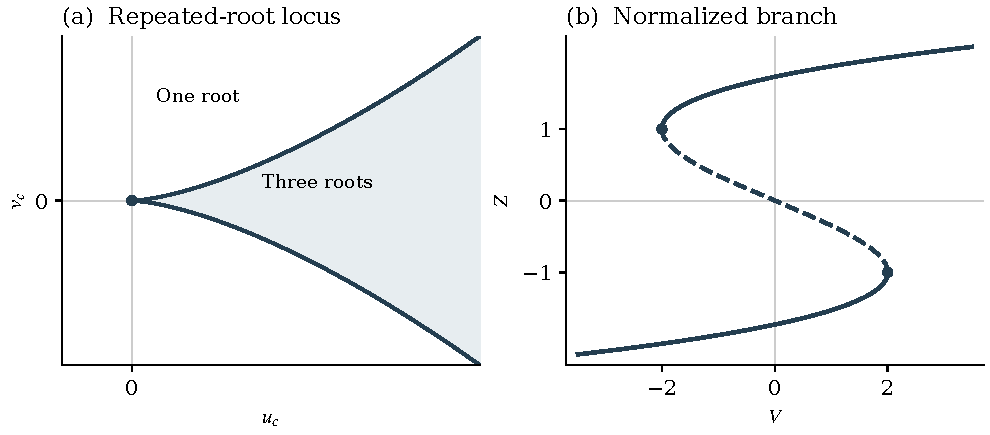
\includegraphics[width=\linewidth]{figures/analytical_branches.pdf}
\caption{Algebraic geometry of coexistence. (a) The two halves of the repeated-root locus in depressed-cubic coefficient space. (b) The universal normalized branch \eqref{eq:normalcubic} for \(u_c>0\). Solid segments have positive determinant at a feasible equilibrium, and the dashed segment has negative determinant. The symbols mark the exact turning values. Python \texttt{code/analytical\_diagram.py}.}
\label{fig:analytic}
\end{figure}

Figure~\ref{fig:analytic} uses only the identities in Proposition~\ref{prop:diagram}. On a feasible branch \(Q'=-a\ell^2\,\dd V/\dd Z\), which explains the determinant labels. The outer branches require the independent trace test of Theorem~\ref{thm:local}.

The local periodic branches can also be drawn without selecting ecological parameters. At a supercritical crossing in Theorem~\ref{thm:enrich}, choose a parameter coordinate \(\lambda\) increasing with the trace and rescale amplitude by the magnitude of the cubic coefficient. The leading radial equation is \(\dot\rho=\rho(\lambda-\rho^2)\). Its positive branch has \(\rho^2=\lambda\) and radial derivative \(-2\rho^2<0\). This gives the attracting branch in Fig.~\ref{fig:cycles}(a).

At the Bautin point in Theorem~\ref{thm:bautin}, its negative quintic radial coefficient and rank-two unfolding give the leading radial polynomial
\[
 \dot\rho=\rho(\eta_1+\eta_2\rho^2-\rho^4).
\]
For \(\eta_2>0\), set \(Z=\rho^2/\eta_2\) and \(U=\eta_1/\eta_2^2\). A positive periodic branch then satisfies \(U=Z^2-Z\). Its radial derivative has the sign of \(1-2Z\). For \(-1/4<U<0\), the two roots have opposite radial stability, while the origin attracts since \(\eta_1<0\). The double root at \(Z=1/2\) gives the cycle fold in Fig.~\ref{fig:cycles}(b). The diagram uses the leading normal forms near onset. The local bifurcation theorems establish the corresponding branches and their stability for the ecological equations.

\begin{figure}[H]\centering
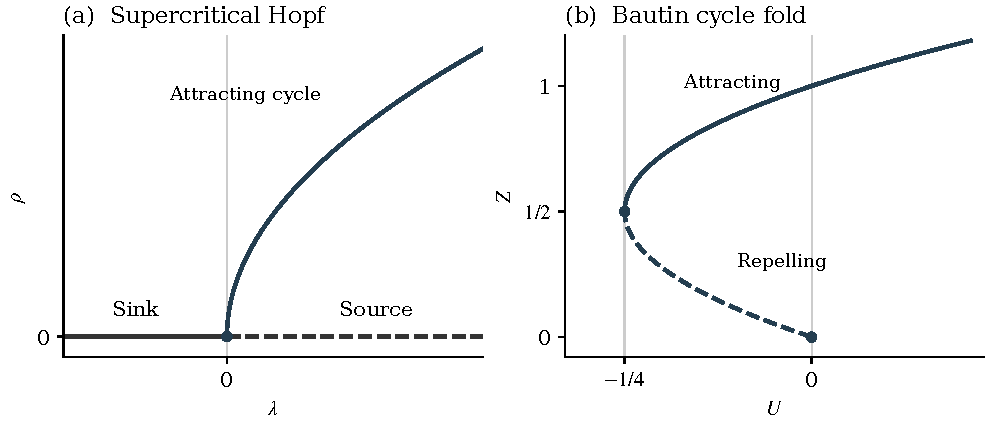
\includegraphics[width=\linewidth]{figures/analytical_cycles.pdf}
\caption{Local periodic branches in normal-form coordinates. Solid branches attract and dashed branches repel in the radial direction. (a) The branch at zero amplitude represents the equilibrium. (b) Positive \(Z\) represents a cycle. On the interval \(-1/4<U<0\) the lower branch is the inner repelling cycle and the upper branch is the outer attracting cycle. Python \texttt{code/analytical\_diagram.py}.}
\label{fig:cycles}
\end{figure}

\begin{table}[H]\centering
\caption{Symbolic constructions and the strict signs that establish their dynamics.}
\begin{tabularx}{\linewidth}{@{}lYY@{}}\toprule
Family & Construction & Analytical certificate\\ \midrule
Bistability & \(0<C<C_{\rm crit}\), \(m_-<m<m_+\), \(L_0>0\) & \(D>M\chi(A)\) excludes cycles and loops\\
Unique cycle & \eqref{eq:shape}, \(h\) small, \(0<D<D_H\) & \(N(s)>0,\ W_L>0\) throughout the strip\\
Dimensional BT & \eqref{eq:btfamily}, \(s\) small & \(a_B>0,\ b_B>0,\ U_B\ne0\)\\
Bautin & \eqref{eq:shape}, \(s\) small, \(h=h_B\) & \(S=0,\ \partial_h S\ne0,\ f_5>0\)\\
Enrichment & \eqref{eq:enrichfamily}, \(m_0\) large & \(\dd T/\dd k>0,\ c_H<0\)\\
\bottomrule\end{tabularx}
\end{table}

\section{Discussion and conclusions}
The quantity \(R\) measures predator growth relative to mortality when rare predators encounter prey at carrying capacity. Extinction occurs at and below the invasion threshold, including the slower inverse-time decay at equality. Above threshold both populations persist. The number of coexistence states then depends on the geometry of \(F+C/x\). The initial increase in prey per-capita growth must be strong enough to outweigh the decline in \(C/x\) before the curve can turn twice. This explains how \(\beta\) affects both invasion and the size of the three-equilibrium region.

If coexistence prey density reaches \(L_0=k-1/\alpha\) or exceeds it, the entropy derivative is strictly negative away from equilibrium. With three simple roots and two outer sinks, either Dulac bound excludes cycles and saddle loops, and the saddle's stable manifold separates the two sink basins. The cycle criterion addresses a different regime. For fixed \(A,s\) on the rising limb, sufficiently small \(h\) makes \(M\) large and the damping-ratio derivative positive throughout the strip when \(0<D<D_H\). The resulting cycle attracts every positive trajectory except the coexistence source.

The focal calculation explains how the local dynamics change across the oscillatory regimes. The cubic focal sign depends on the first derivative of the ratio \(N/\Q\) at the critical equilibrium. When that derivative vanishes on the family in Theorem~\ref{thm:bautin}, its next odd contribution determines the direction of the cycle fold. In the original parameters, the BT construction identifies a family near small positive prey densities, and the enrichment theorem shows exactly how a positive capacity derivative can destabilize coexistence. These mechanisms connect the biological parameters to local oscillations without estimating a trajectory.

\begin{table}[H]\centering
\caption{Scope of the analytical conclusions.}
\begin{tabularx}{\linewidth}{@{}lYY@{}}\toprule
Question & Established result & Remaining problem\\ \midrule
Coexistence & Necessary and sufficient invasion and multiplicity thresholds & Nonlinear unfolding at a nilpotent triple root\\
Basins & Complete partition under the global exclusion hypotheses & Classification when the divergence changes sign\\
Cycles & Global one-cycle family and a local two-cycle wedge & Global counts away from the proved regions\\
Enrichment & Supercritical destabilization on a dimensional family & Continuation and amplitude far from onset\\
\bottomrule\end{tabularx}
\end{table}
\bibliographystyle{elsarticle-harv}
\bibliography{references}
\end{document}
